\label{chap:konstruktion}
\chapter{Design und Konstruktion}
\section{Verschiedene Segelbootstypen}
Segelboote weisen eine jahrtausendalte Entwicklungsgeschichte auf. Sie kommen daher in einer unüberschaubaren Zahl von unterschiedlichen Ausgestaltungen vor, die vom einfachen, mit einem Segel versehenen Floss aus Schilf über mehrmastige Karavellen aus Holz, Freizeitjachten aus Aluminium oder Kunststoff bis zur Hightech Rennjacht aus Carbonfasern reicht. Trotz dieser Diversität lassen sich alle Segelboote anhand von drei Hauptmerkmalen (i) Rumpfzahl (ii) Segelart und (iii) Kielart kategorisieren.
\subsection{Rumpfzahl}
Die erste und einfachste Unterscheidung der verschiedenen Segelboottypen erfolgt anhand der Zahl der Rümpfe. Wenn man sich ein Segelboot vorstellt, denkt man an ein Einrumpfboot (Mono Hull). Es gibt aber auch Mehrrumpfboote (Multi Hull) mit zwei oder drei Rümpfen. Bekannte Vertreter sind Katamaran und Trimaran.
\subsection{Segelart}
Segel lassen sich grob in flexible und feste Segel einteilen. Flexible Segel bestanden ursprünglich aus Segeltüchern, die aus Wolle hergestellt wurden. Heute werden für Segeltücher fast ausschliesslich verschiedenen Kunstfasern wie Nylon, Polyester, Kevlar, aber auch Carbon verwendet, die oft laminiert werden. 

Festsegel sind steif und fristen ein Nischendasein. Sie finden sich bisher nur bei experimentellen Booten und Schiffen in zwei sehr unterschiedlichen Bereichen. Einerseits können damit grosse Kreuzfahrt- oder Containerschiffe ausgerüstet werden, um deren Energie- und Umwelteffizienz zu verbessern. Dabei kann durch die Verwendung von zusammengesetzten Komposit-Paneelen die mit dem Einsatz textiler Standardsegel verbundene Grössenbeschränkung überwunden werden. \cite{redaktion_bv-grundsatz-zulassung_2022} Andererseits werden Prototypen für autonome Segelboote und Segelbootdrohnen fast ausschliesslich mit Festsegeln ausgerüstet. Diese Boote weisen Längen von 2 m bis 20 m auf und die technischen Grössenbeschränkungen textiler Segel sind bei ihnen daher ohne Relevanz. Ihr Hauptvorteil gegenüber flexiblen Segeln ist die vergleichsweise einfache Segelführung im Betrieb. Festsegel bestehen bei kommerziellen Projekten aus Verbundwerkstoffen und bei nicht-kommerziellen Projekten meistens aus expandiertem Polystyrol (EPS), das unter dem geschützten Handelsnamen \enquote{Styropor} bekannt ist. Der in Form gebrachte Segelkörper wird dabei zum Schutz fast immer mit glasfaserverstärktem Kunststoff (GFK) (umgangssprachlich als Fiberglas bekannt) oder anderen Kunststoffen ummantelt.
\subsection{Kielart}
Segelboote lassen sich in Kiel und Schwertboote unterteilen. Der Kiel ist der unterste Teil eines Bootrumpfes. Ein grosser Teil der Segelboote, insbesondere die grösseren Boote, verfügen über einen Balastkiel. Das ist eine schwerere, aus Gusseisen oder Blei bestehende Kielflosse. Der Balastkiel macht etwa ein Drittel bis die Hälfte des gesamten Bootsgewichts aus. Der Kiel dient beim Segelboot zur Verminderung der seitlichen Abdrift und sorgt für Gewichtsstabilität (siehe \ref{subchap:exkurs}).

Keinen Kiel haben Flachbodensegelschiffe wie Jollen oder bestimmte Kuttertypen, die in Flachgewässern operieren. Auch die Mehrrumpfboote verfügen über keinen Kiel. Zur Vermeidung der Abdrift verfügen diese Segelboote anstelle eines Kiels über ein Schwert. Ein Schwert ist eine parallel zur Fahrtrichtung vorgesehene senkrechte Platte aus Stahl, Holz oder glasfaserverstärktem Kunststoff. Das Schwert ist fast immer beweglich ausgestaltet, kann also eingezogen oder eingeklappt werden. Für die Stabilität von Schwertsegelbooten sorgt allein ihre Form.
\section{Exkurs zur Stabilität von Segelbooten}
\label{subchap:exkurs}
Der Begriff Stabilität steht im Schiffbau für die Eigenschaft eines Bootes, eine aufrechte Schwimmlage einzunehmen und beizubehalten oder sich selbstständig wieder aufzurichten, wenn ein krängendes Drehmoment auf das Boot einwirkt oder einwirkte. Krängung ist die Neigung eines Schiffs um seine Längsachse. \cite{noauthor_stabilitat_2023}  Umgangssprachlich wird Krängung auch als Schräglage bezeichnet.
\begin{figure}[H]
    \centering
    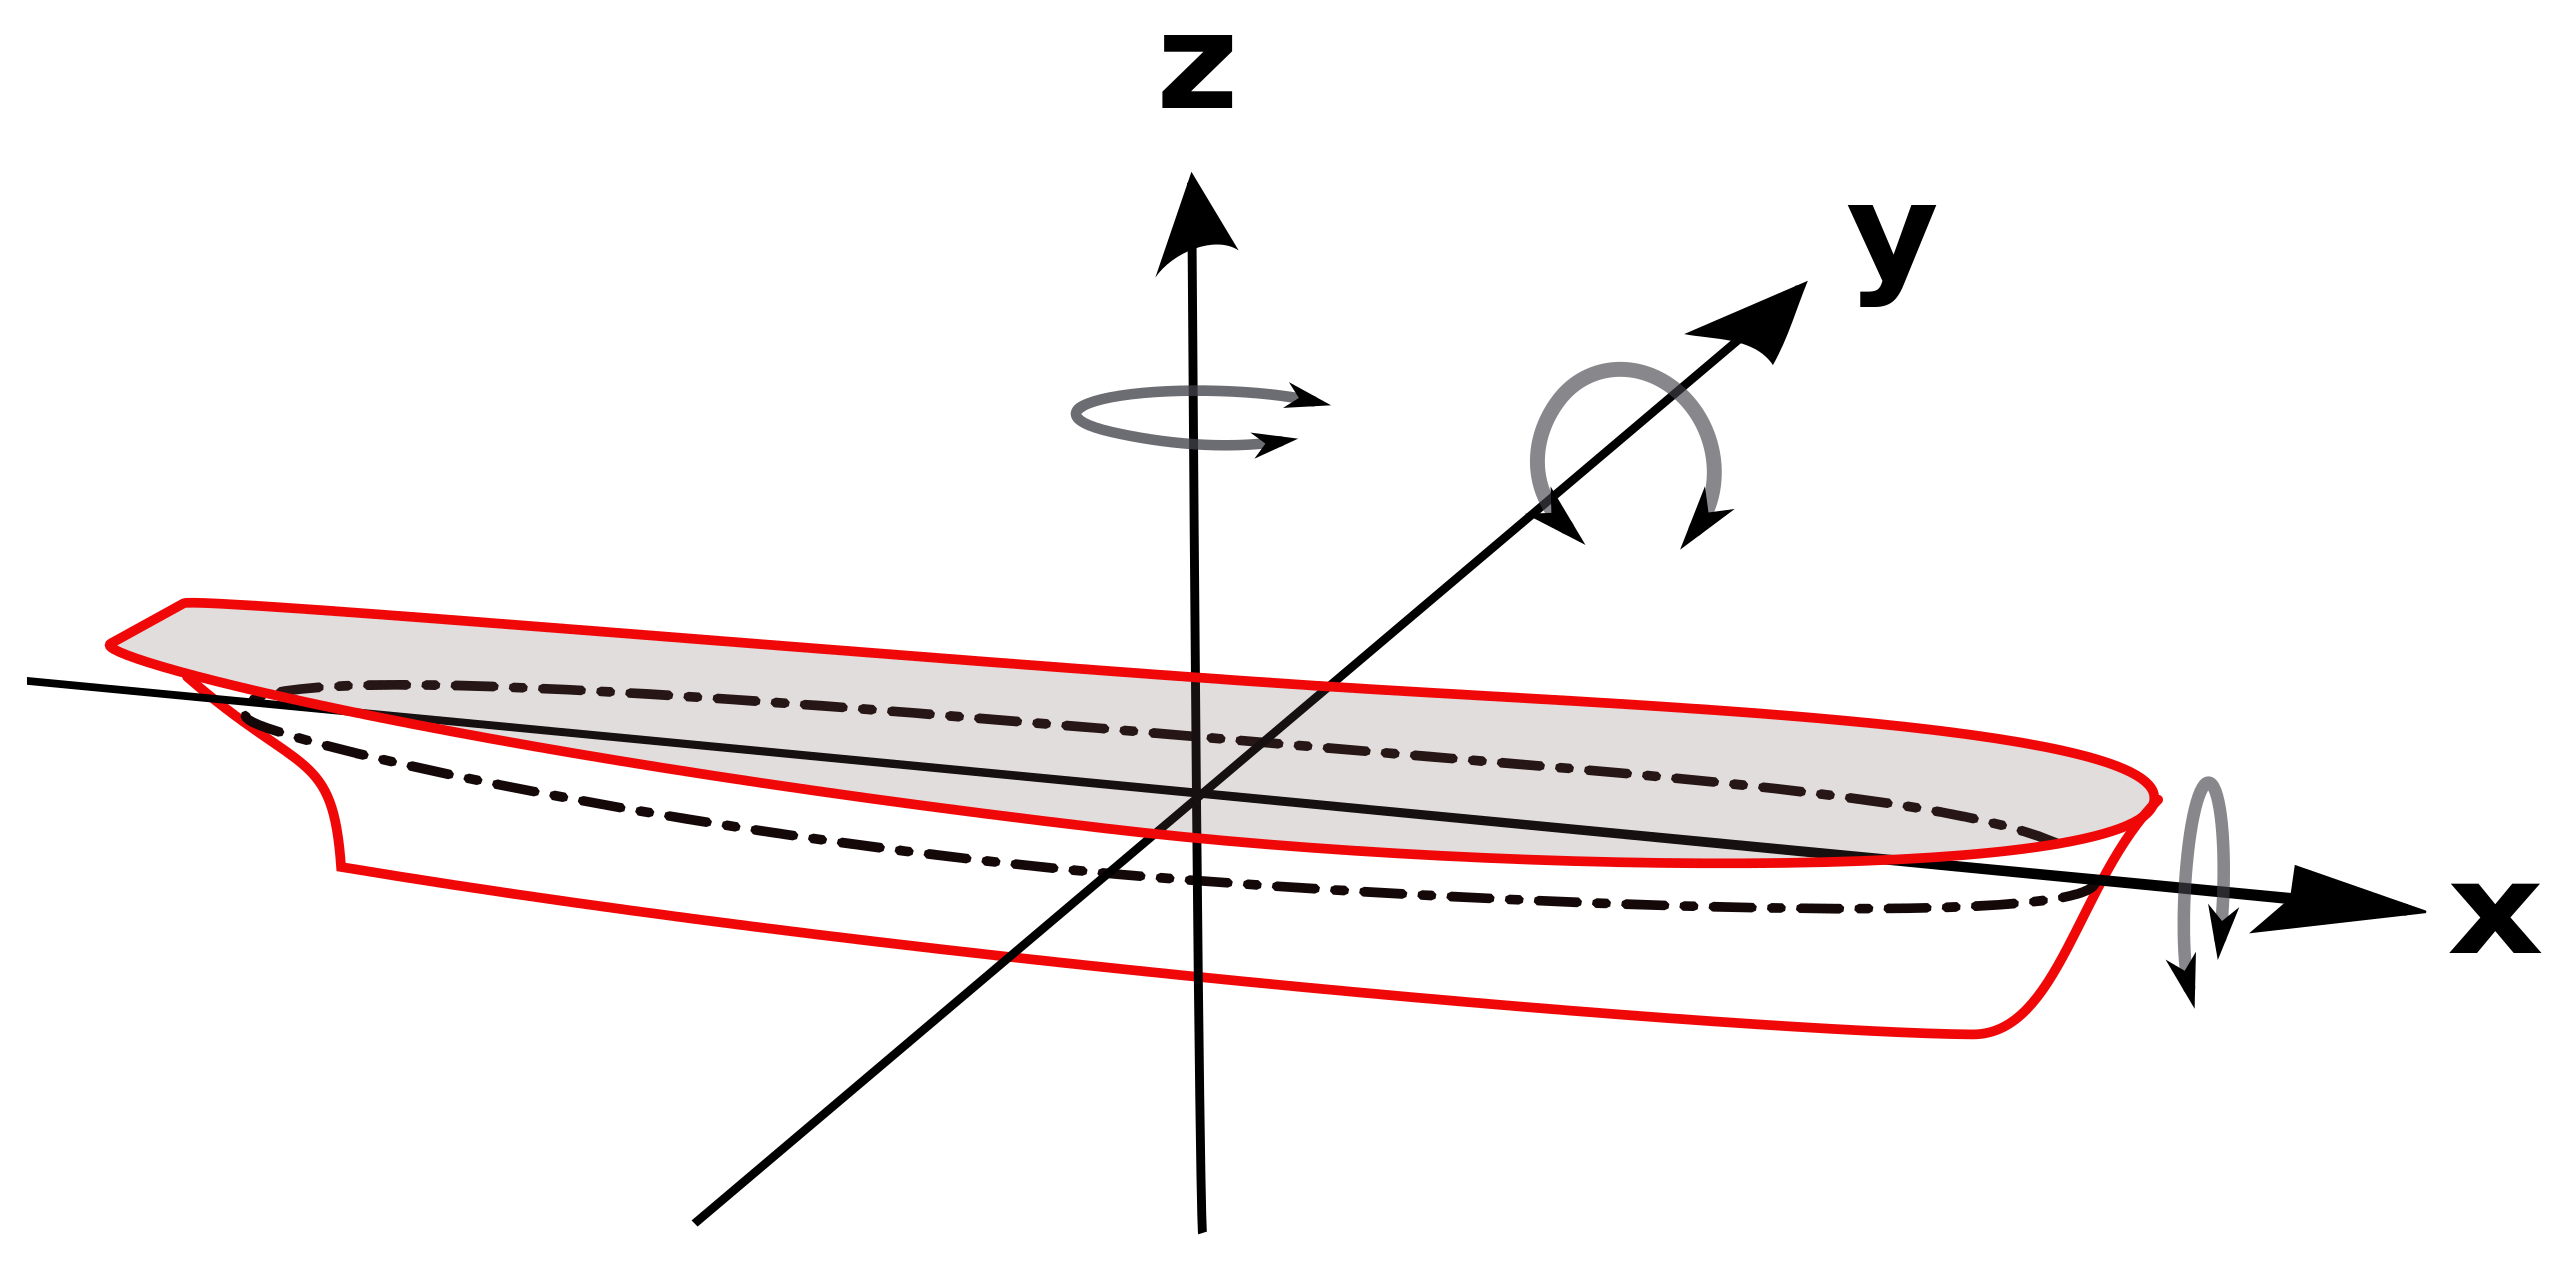
\includegraphics[width=0.75\linewidth]{assets/Achsen_Schiffsbewegung.svg.png}
    \caption{Krängung}
    \label{fig:enter-label}
\end{figure}
Bei geringer Stabilität besteht die Gefahr des Kenterns. Kentern bezeichnet in der Nautik einen Unfall, bei dem ein Wasserfahrzeug seitlich umkippt, wenn dessen Krängung durch Wind, Wellengang oder Verlagerung von Fracht, Ausrüstung oder Mannschaft den Kenterwinkel erreicht. Dreht sich das Schiff danach weiter um seine Längsachse, so spricht man von Durchkentern. Ein gekentertes Schiff kann Wasser aufnehmen und in der Folge sinken.  

Autonome Segelboote dürfen nicht kentern, da sie sonst ihr Ziel nicht mehr erreichen können. Sie müssen daher über eine sehr hohe Stabilität verfügen.

Die Stabilität eines Bootes wird durch drei Parameter bestimmt: seinen Gewichtsschwerpunkt, seinen Auftriebsschwerpunkt sowie die sich aus diesen ergebende sogenannte metazentrische Höhe.\cite{noauthor_stabilitat_2023-1}  
\begin{itemize}
    \item Der Gewichtsschwerpunkt steht für die gesamte, in einem Punkt konzentrierte, nach unten wirkende Gewichtskraft eines Bootes. Seine Lage innerhalb des Bootes verändert sich bei einer Krängung nicht, solange alle Massen im Boot unverändert an ihrem Ort verharren.
    \item Der Auftriebsschwerpunkt (auch Form- oder Verdrängungsschwerpunkt genannt) steht für die gesamte, in einem Punkt konzentrierte, nach oben wirkende Gewichtskraft des verdrängten Wassers. Seine Lage ändert sich bei einer Krängung, weil sich durch die Rumpfform auch die „Form“ des verdrängten Wassers ändert.
    \item Als metazentrische Höhe wird der entlang der Körpervertikalen gemessene Abstand des Metazentrums vom Gewichtsschwerpunkt bezeichnet. Das Metazentrum eines Schiffs entspricht dem Aufhängungspunkt eines Stabpendels. Während aber dessen Aufhängunspunkt gleichzeitig auch der Drehpunkt ist, liegt beim Schiff die Drehachse immer auf der Wasseroberfläche.\cite{noauthor_metazentrische_nodate}
\end{itemize}
\begin{figure}[H]
    \centering
    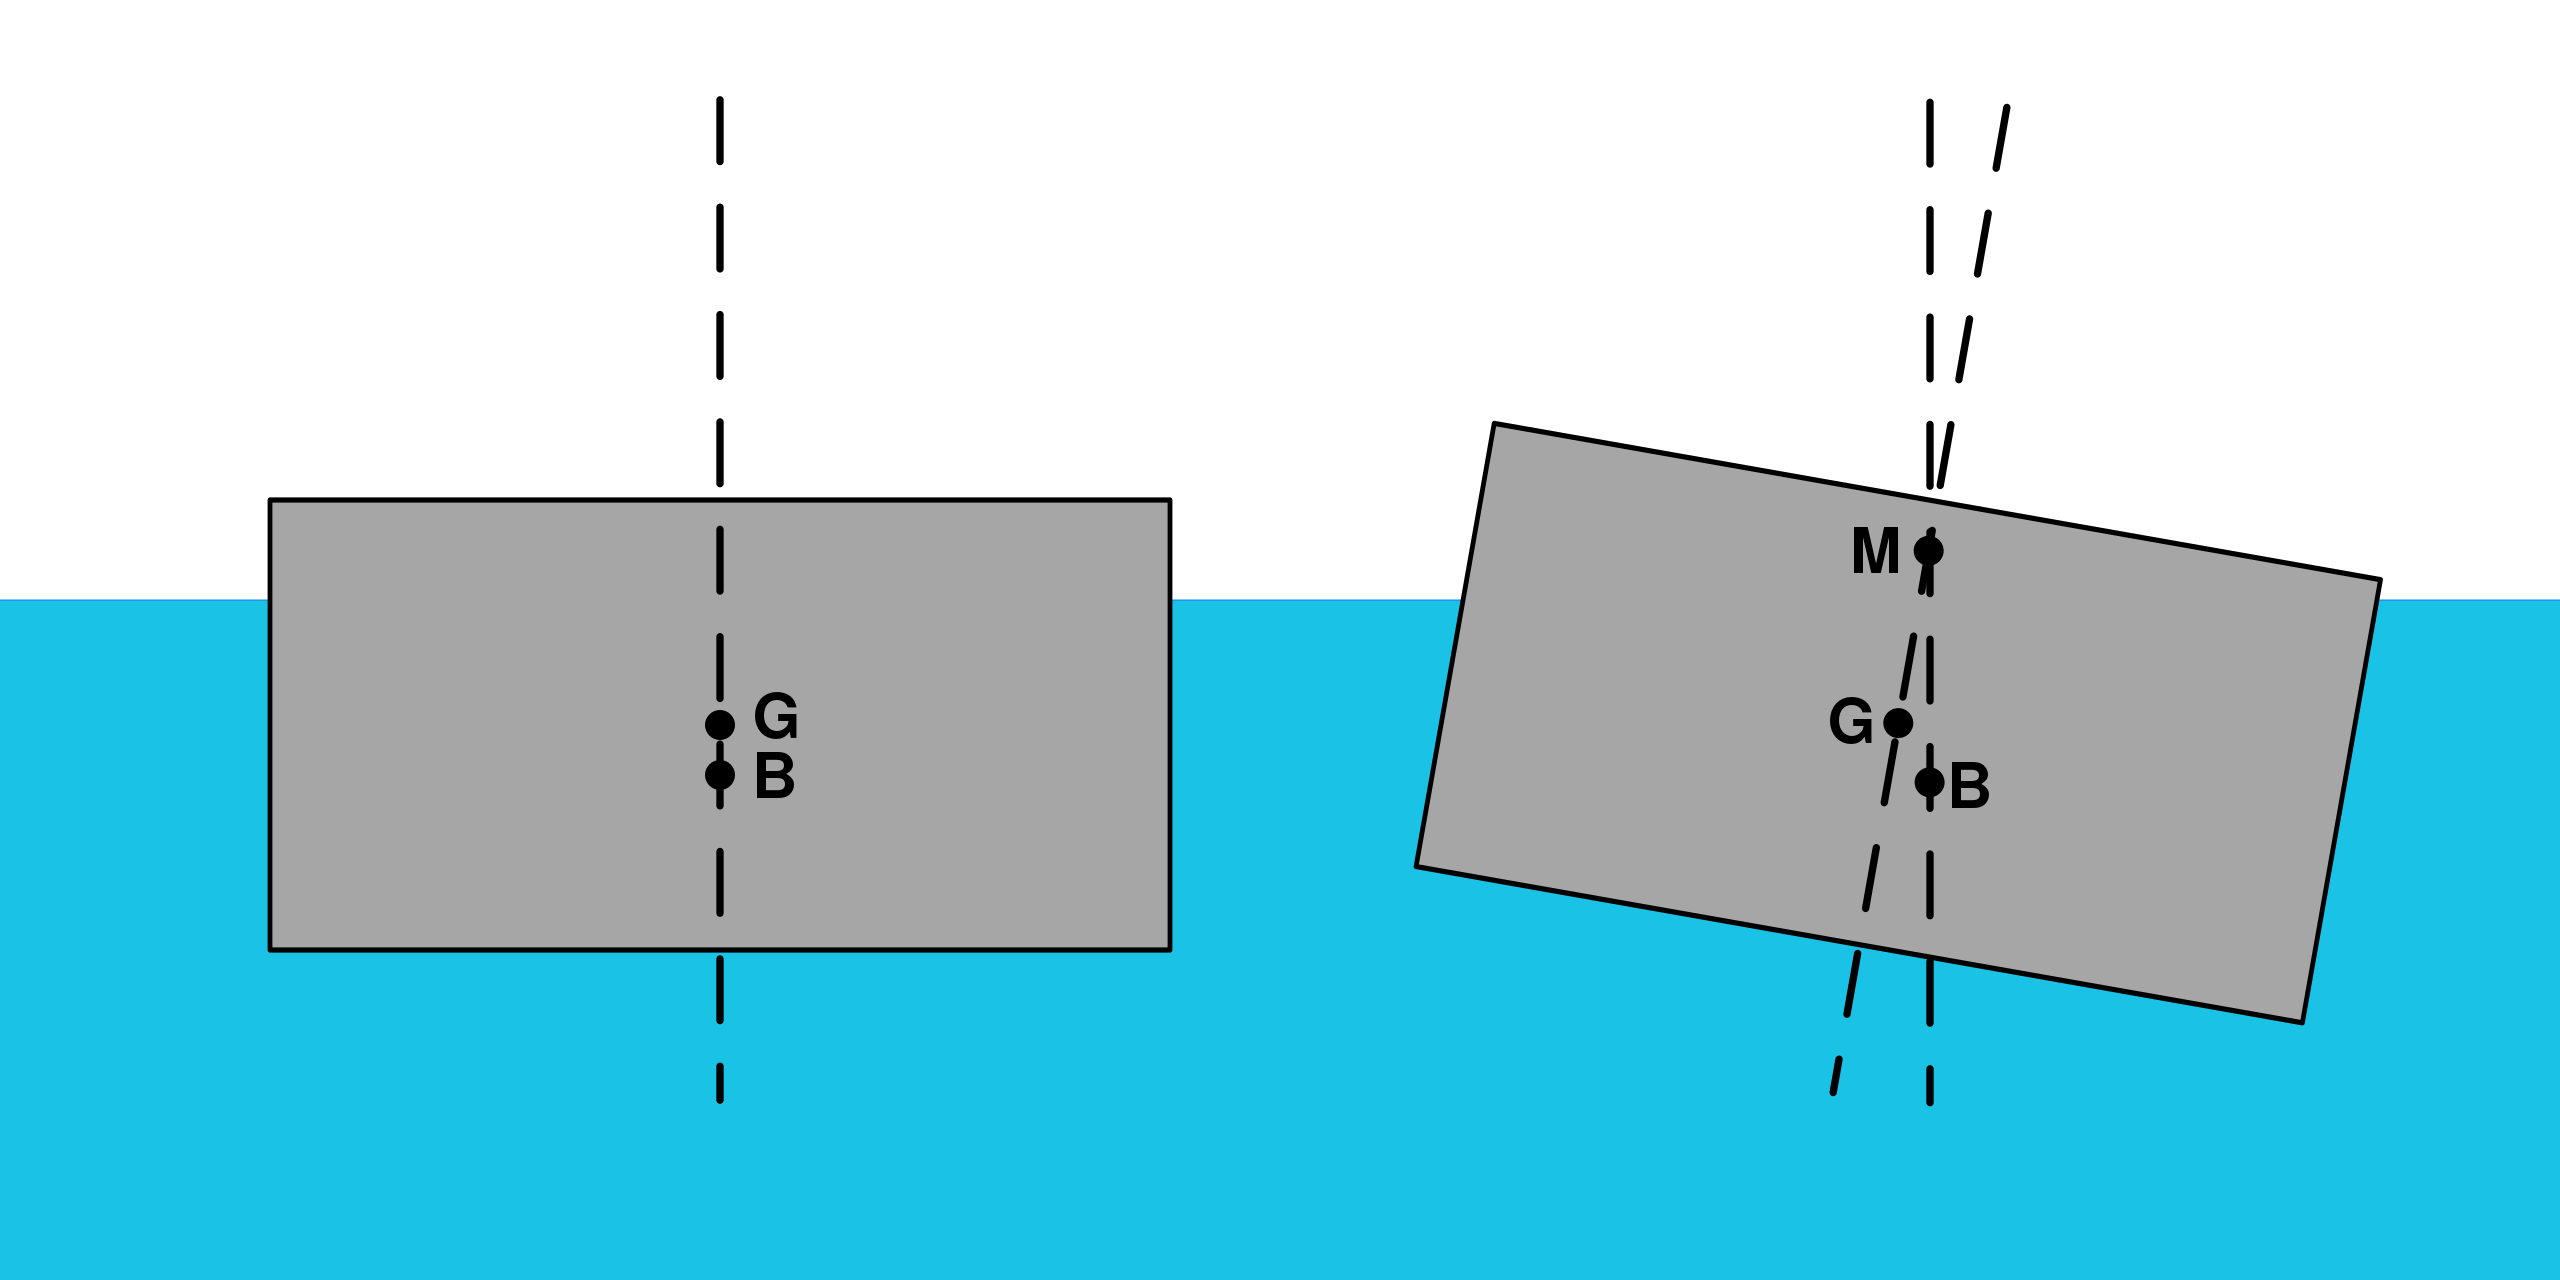
\includegraphics[width=0.75\linewidth]{Metacentriskhojd-svg.svg.png}
    \caption{Lage des Gewichtsschwerpunkt (G), Auftriebsschwerpunkt (B) und Metazentrum (M) bei aufrechtem sowie gekrängtem Boot }
    \label{fig:enter-label}
\end{figure}
Bei aufrechter Schwimmlage eines Schiffes liegt der Gewichtsschwerpunkt exakt vertikal über dem Auftriebsschwerpunkt. Führt ein äusserer Einfluss aber zu einer Krängung des Schiffs, verändert sich die Lage des Gewichtsschwerpunkts auf der horizontalen Achse. Gewichtsschwerpunkt und Auftriebsschwerpunkt stehen damit nicht mehr senkrecht übereinander. Dadurch entsteht ein aufrichtendes Drehmoment, welches das Boot bei Wegfall des krängenden Einflusses in seine Ausgangslage zurückführt.

Zur Bewertung der Stabilität eines Schiffes müssen die folgenden drei Parameter bekannt sein: 
\begin{itemize}
    \item Die Anfangsstabilität (die sogenannte metazentrische Anfangshöhe),
    \item der Stabilitätsumfang und
    \item die Fläche unter der Hebelarmkurve.
\end{itemize}
Die metazentrische Anfangshöhe ist der Parameter für den aufrichtenden Hebelarm. Mit dem Stabilitätsumfang wird die rechnerische Krängung des Schiffes in Winkelgraden bis zum Kenterpunkt bezeichnet und mit der Hebelarmkurve wird der jeweilige aufrichtende Hebelarm über den vollen Krängungsbereich bis zum Kenterpunkt des Bootes grafisch dargestellt.
Der Hebelarm wächst bei zunehmender Krängung zunächst steil und dann immer flacher an. Bei noch stärkerer Krängung wird er wieder geringer, bis er schliesslich den Kenterpunkt (C) erreicht. Dieser liegt da, wo der Gewichtsschwerpunkt über den Auftriebsschwerpunkt hinauswandert. \cite{noauthor_stabilitat_2023}

\begin{figure}[H]
    \centering
    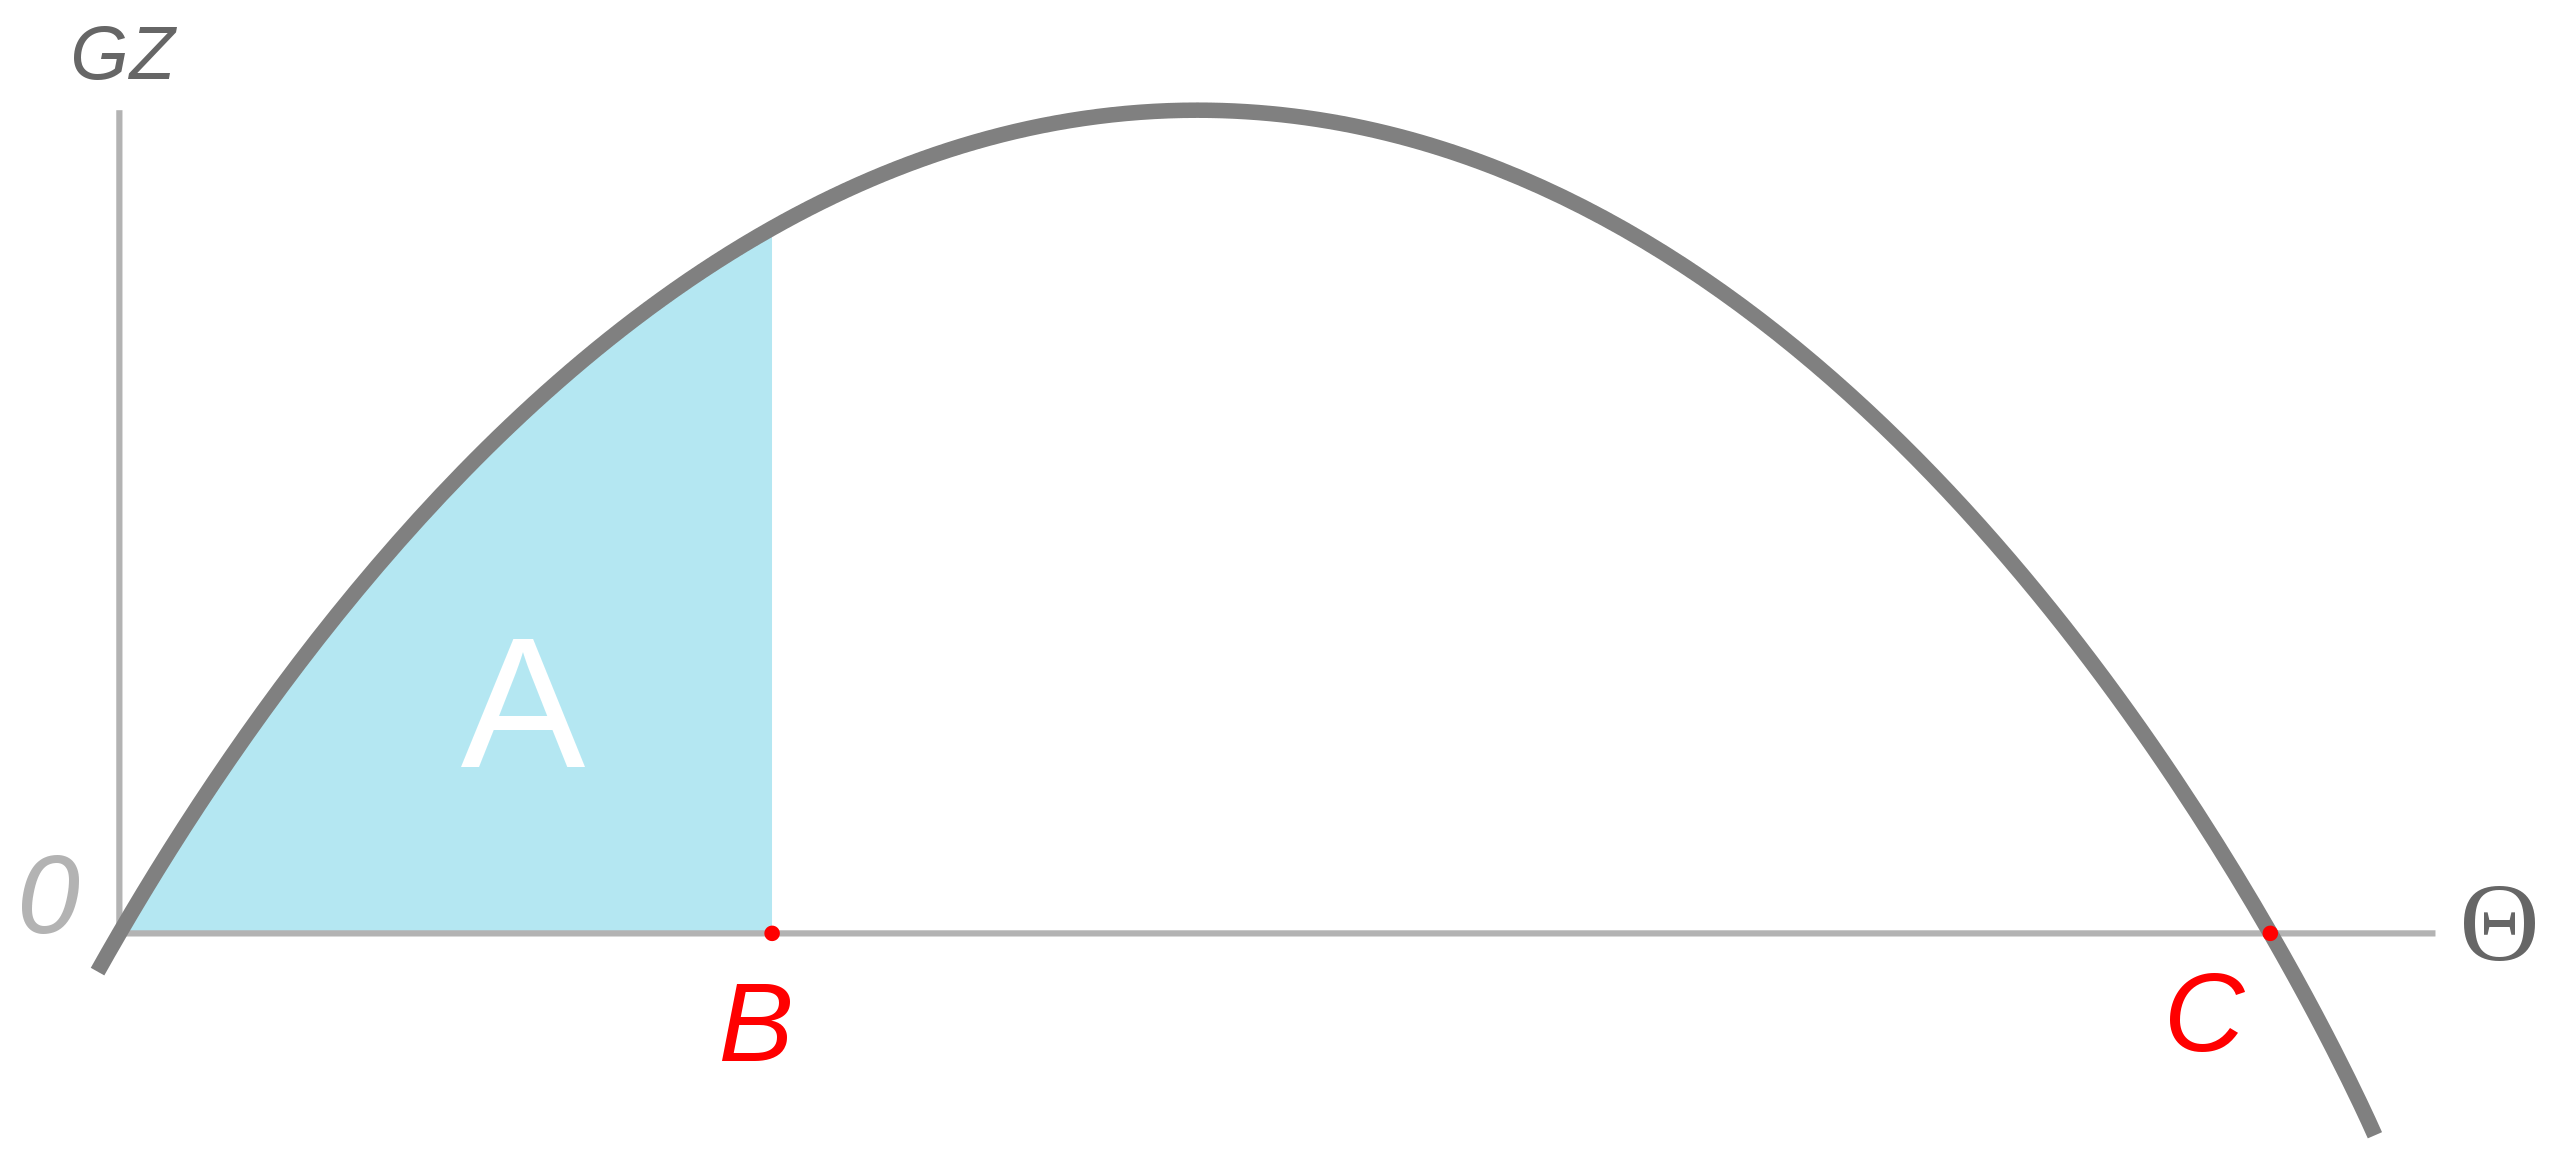
\includegraphics[width=0.5\linewidth]{Stability_curve_NT.svg.png}
    \caption{Hebelarmkurve}
    \label{fig:enter-label}
\end{figure}
Bei Segelbooten sind die Überlegungen zur Stabilität besonders wichtig, da sie dem Wind mit ihrem Segel eine sehr grosse Angriffsfläche bieten. Ohne geeignete Gegenmassnahmen kippen sie schon bei geringen Windstärken um. Entscheidend für die Stabilität eines Segelbootes sind dabei die Rumpfform und Gewichtsverteilung des Bootes. Die Stabilität eines Boots kann erhöht werden, wenn die Krängung durch eine der zwei folgenden Massnahmen ausgeglichen wird:
\begin{itemize}
    \item Gewichtsstabilität – ein tief liegender Ballastkiel zwingt das Boot wieder in die aufrechte Lage (sogenanntes Stehaufmännchen-Prinzip).
    \item Formstabilität – die Form des Rumpfes begünstigt eine Rückkehr in die Ausgangslage.
\end{itemize}
\paragraph{Gewichtsstabilität}
Ein Ballastkiel wirkt der Krängung eines Bootes als Gegengewicht entgegen. Er enthält bis zur Hälfte der Masse des Segelschiffs und bewirkt damit ein aufrichtendes Moment. Eine Krängung von 20 bis 45 Grad ist bei Segelbooten aber durchaus normal und stellt keine Gefahr für das Schiff dar. Dies ergibt sich ohne weiteres aus der unten stehenden Abbildung. Dabei steht G für den Gewichtsschwerpunkt (Schwerpunkt des Bootes) und A für den Auftriebsschwerpunkt (Schwerpunkt der verdrängten Wassermasse). Mit zunehmender Krängung wandert der Gewichtsschwerpunkt immer weiter nach aussen. Damit erhöht sich aber auch das aufrichtende Drehmoment. 
\begin{figure}[H]
    \centering
    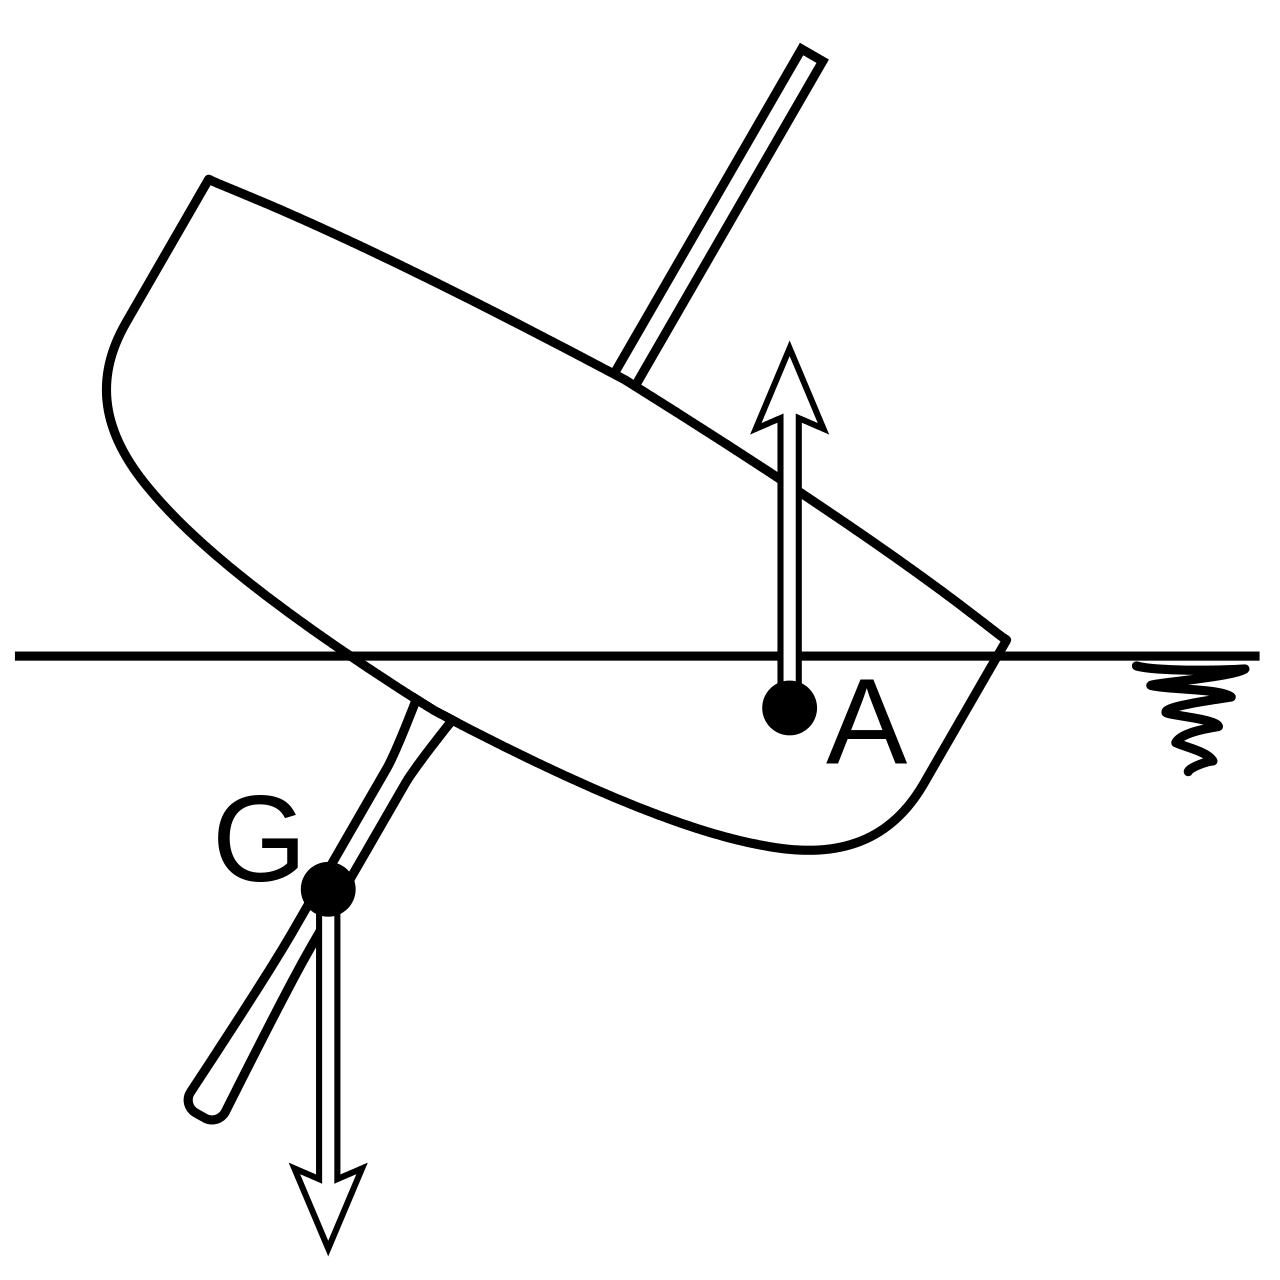
\includegraphics[width=0.25\linewidth]{Segeln_Gewichtsstabilitaet.svg.png}
    \caption{Gewichtsstabilität durch Ballastkiel }
    \label{fig:enter-label}
\end{figure}
Es gibt Segelschiffe die sich selbst bei einer Krängung von mehr als 120 Grad selbstständig wieder aufrichten. Sie gelten daher als kentersicher, denn sie können nur durch sehr hohen Wellengang mit dem Kiel nach oben gedreht werden. Nimmt der Bootskörper dabei viel Wasser auf, sinken sie wegen des hohen Ballastgewichts. 
\paragraph{Formstabilität}
Im Unterschied zu Kielbooten sind Schwertboote kaum gewichtsstabil, sondern überwiegend formstabil. Ihr leichtes Schwert hat nämlich keinen nennenswerten aufrichtenden Effekt. Wie die unten stehende Abbildung zeigt, ist für die Formstabilität die Lage des Auftriebsschwerpunkts A ausschlaggebend. Wenn sich ein Boot in einer aufrechten Lage befindet, wird auf beiden Seiten des Rumpfes gleich viel Wasser verdrängt. A befindet sich dann mittig im Rumpfquerschnitt und es entsteht kein Drehmoment. Mit zunehmender Krängung wird Wasser zunehmend nur noch auf einer Seite des Rumpfes verdrängt. Dadurch wandert A immer mehr nach aussen und es entsteht ein Drehmoment. Je breiter das Boot ist, desto weiter kann A nach aussen wandern und desto stärker ist das aufrichtende Drehmoment. 
\begin{figure}[H]
    \centering
    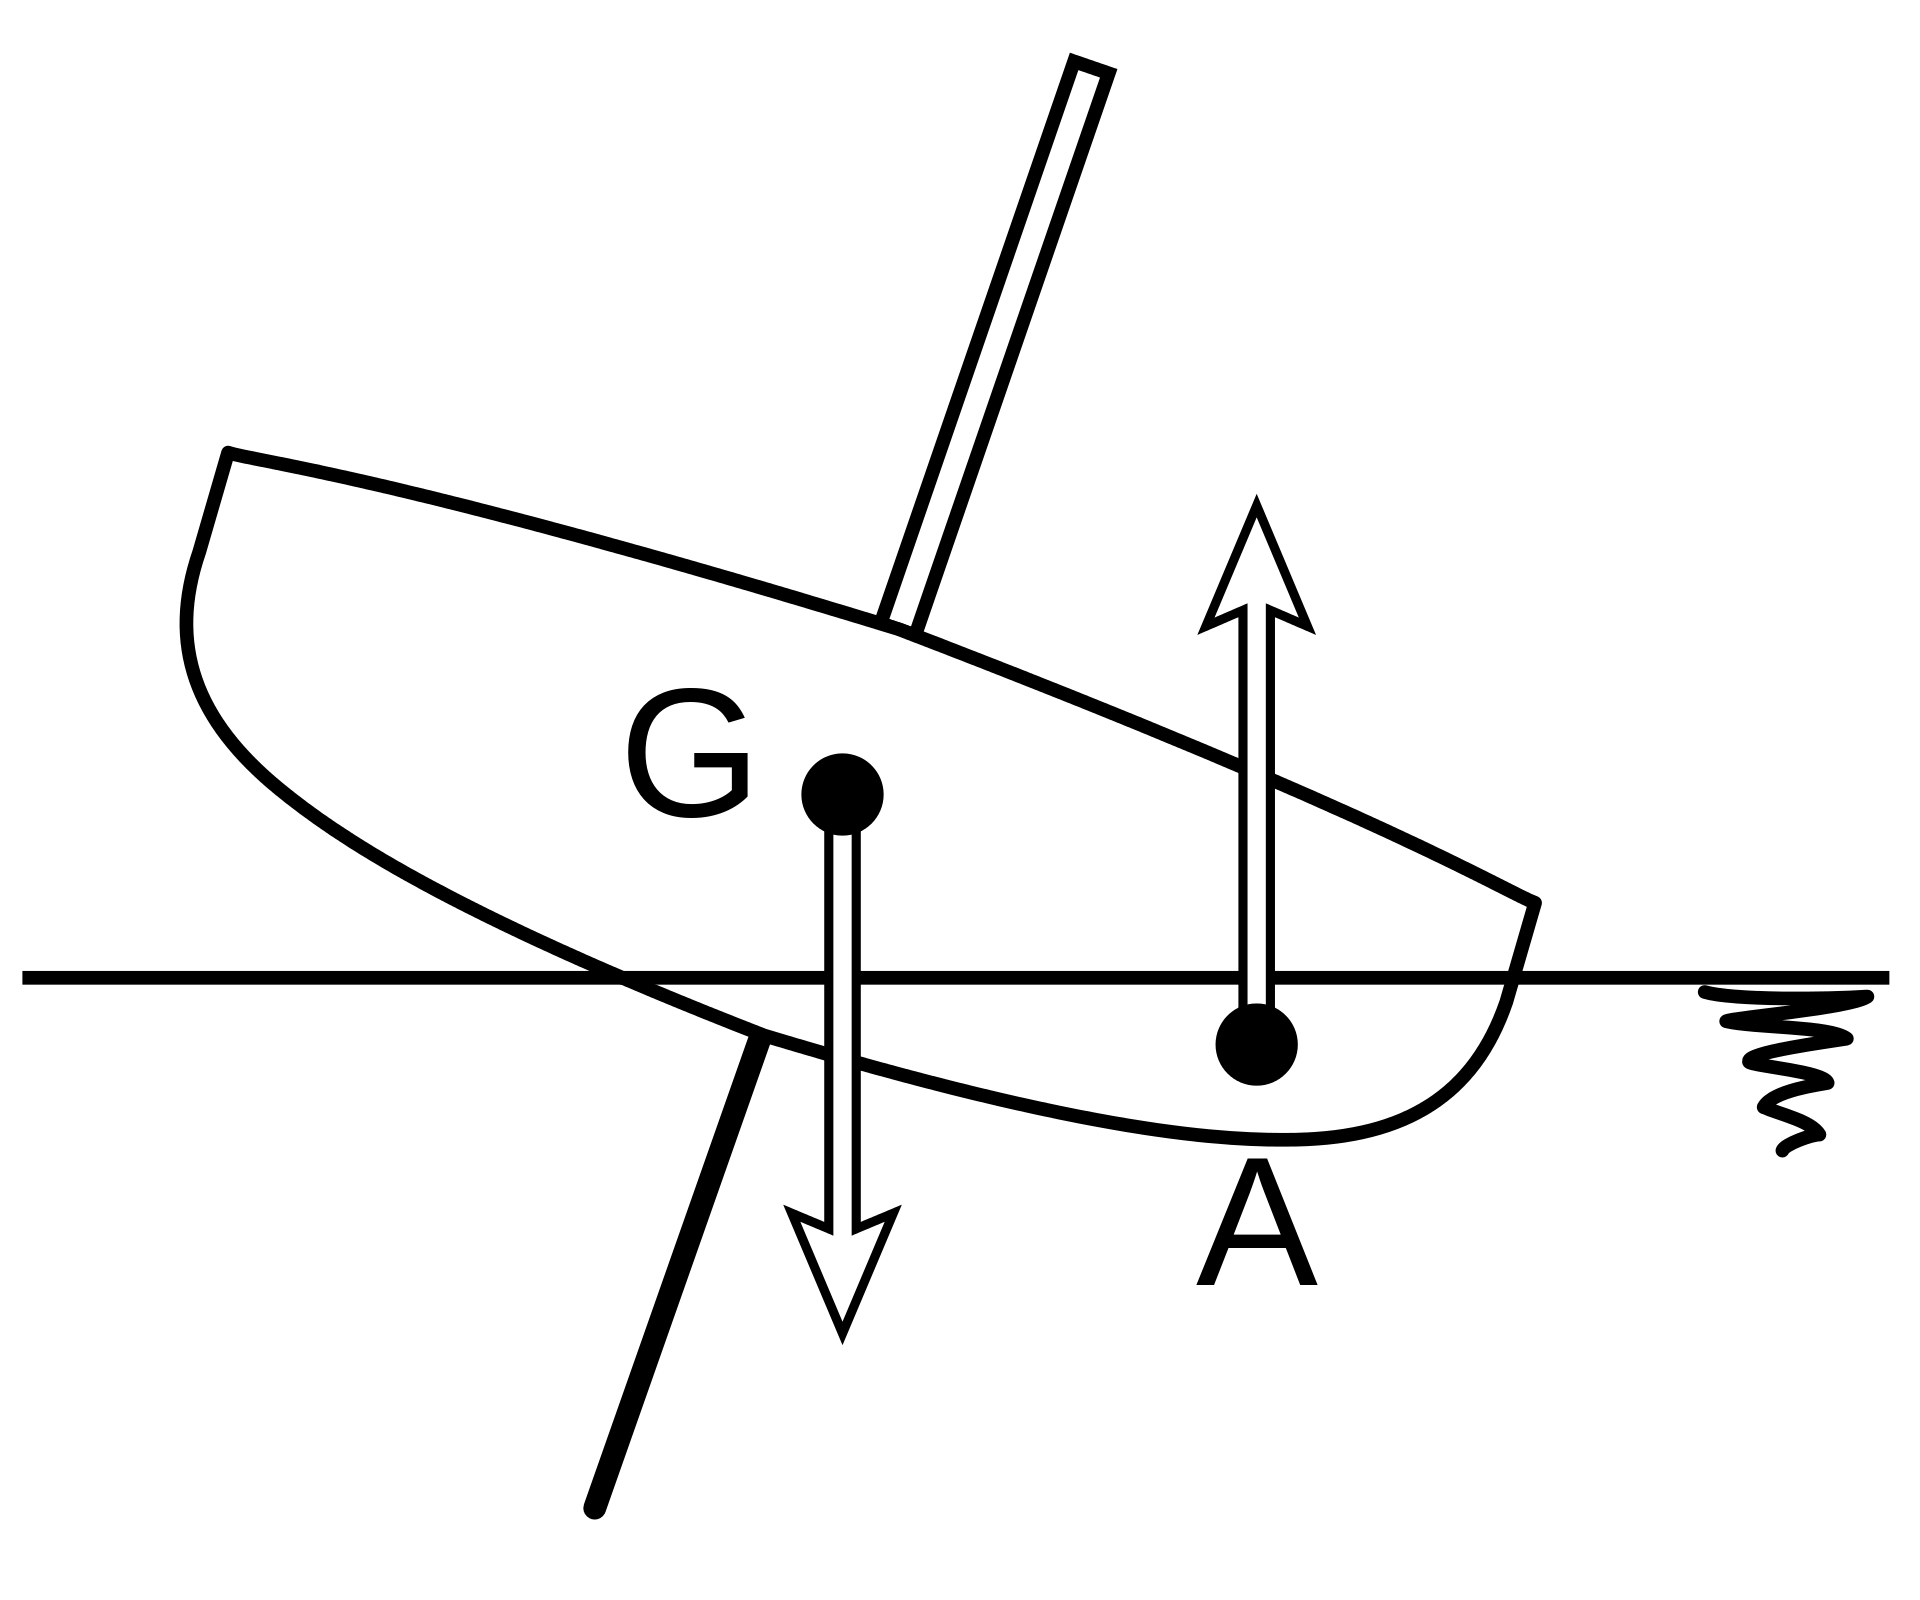
\includegraphics[width=0.5\linewidth]{Segeln_Formstabilitaet.svg.png}
    \caption{Formstabilität }
    \label{fig:enter-label}
\end{figure}
Wenn die Krängung aber zu gross wird, nimmt das Drehmoment wieder ab, weil dann der Rumpf kippt und A wieder näher bei der Mitte liegt. Eine leichte Krängung wird daher durch das kräftige aufrichtende Drehmoment kompensiert, während eine zu starke Krängung zum Kentern des Bootes führt. Katamarane kentern erst, wenn die Krängung 90 Grad erreicht. 

Bei Schwertbooten wird die Stabilität durch die entsprechende Formgebung des Rumpfquerschnittes erreicht, während sie bei Kielbooten von der Masse und der Länge des Kiels bestimmt wird. Schwertboote besitzen bei leichter Krängung aufgrund ihrer Formstabilität ein sehr hohes aufrichtendes Moment. Dieses aufrichtende Moment nimmt aber mit zunehmender Krängung stark ab, sodass es zur Kenterung kommen kann. Bei Kielbooten ist es genau umgekehrt, bei leichter Krängung ist das aufrichtende Moment gering und nimmt bei zunehmender Krängung zu, sodass sie kaum kentern können bzw. sich nach einer Kenterung von alleine wieder aufrichten. 
\cite{noauthor_schwertboot_2023}
\section{Wahl des Bootstypus}
\subsection{Wahl der Segelart}
Ausgangspunkt für die Wahl des Bootstypus für das vorliegende Projekt bildet der Entscheid über das zu verwendende Segel. Da sich das Segelboot autonom bewegen können muss, fällt dieser Entscheid leicht, denn nur mit einem Festsegel lässt sich die Neigung, flexibler Segel zu flattern, vermeiden. 

Die Verwendung eines flexiblen Segels würde den Einbau einer sehr 
aufwendigen und auch fehleranfälligen Mechanik zur automatischen Trimmung des Segels mit Leinen und Rollen erfordern. Selbst wenn die Entwicklung einer Trimmmechanik gelingen würde, müsste das Segelboot zusätzlich in die Lage versetzt werden, ein loses (also ein flatterndes) oder zu strammes Segel selbstständig zu erkennen und entsprechende Steuerbefehle an die Segeltrimmmechanik zu senden. Idealerweise müsste das Segelboot aber nicht nur jedes Abweichen von der idealen Segelform selbstständig erkennen, sondern es müsste auch die negativen Auswirkung von Ruderbewegungen, Windböen oder starkem Wellenschlag auf die ideale Segelform selbstständig antizipieren können. 

Das würde erfordern, dass entweder direkt im Segel Sensoren verbaut würden oder dass das Segel optisch mittels einer oder mehrere Kameras erfasst würde. Aus diesen Daten würde dann in Echtzeit in einem ersten Schritt der Ist-Zustand des Segels berechnet, dieser in einem zweiten Schritt mit dem Idealzustand verglichen, in einem dritten Schritt der Anpassungsbedarf berechnet, in einem vierten Schritt die notwendige Massnahme ermittelt (eine Verlängerung oder eine Verkürzung der Leinen (Schotten) und/oder ein Steuereingriff am Ruder) und in einem letzten Schritt der entsprechende Befehl an die Trimm- und/oder Steuermechanik übermittelt. 

Die Entwicklung einer solchen Trimmautomatik für eine flexibles Segel sprengt den Rahmen einer Maturaarbeit bei weitem, selbst wenn sie als selbstständige Arbeit vorgesehen würde. Bei einem autonomen Segelboot dieser Klasse muss daher der Entscheid zwingend zugunsten eines Festsegels lauten.
\subsection{Wahl der Rumpfzahl}
Ein Festsegel kann sowohl mit Einrumpfbooten als auch mit Mehrrumpfbooten eingesetzt werden, womit der Entscheid über die Rumpfzahl nicht durch den Entscheid über die Segelart antizipiert wird.  

Für das vorliegende Projekt wird eine Einrumpfkonstruktion vorgezogen, da diese einfacher zu realisieren ist. Doppelrumpfboote verfügen über keinen Kiel und bieten damit keine Gewichtsstabilität. Sie sind nicht kentersicher und scheiden aus. Trimarane können theoretisch mit einem Kiel versehen werden, womit sie Gewichts- und Formstabilität bieten. Sie erfordern aber einen sehr hohen konstruktiven Aufwand, ohne für die Zwecke dieses Projektes gegenüber einem Einrumpfboot (mit einem Kiel) einen entscheidenden Vorteil zu bieten. 
\subsection{Kiel oder Schwertboot}
Unter 4.2 werden Kiel- und Schwertboote unter dem Aspekt der Stabilität betrachtet. Dabei zeigt sich, dass Schwertboote im Gegensatz zu Kielbooten nicht kentersicher konstruiert werden können. Damit scheidet eine Schwertbootskonstruktion für die vorliegenden Zwecke aus.

Bei der Konstruktion des Bootes muss eine hohe Gewichtsstabilität erreicht werden. Da dieser für autonome Fahrten in Binnengewässern nicht sehr lang vorgesehen werden kann, wird er mit einem sehr hohen Balastgewicht versehen.
\subsection{Ergebnis des Auswahlverfahrens zum Bootstyp}
Nach Abschluss des Auswahlverfahrens zum Bootstyp steht fest, dass ein einrumpfiges Kielboot mit einem Festsegel konstruiert wird.
\section{Grundmaterialentscheid }
Boote können aus diversen Materialien gebaut werden. Der Bau eines Bootskörpers aus Stahl oder Aluminium scheidet aber von vornherein aus, weil kein Zugang zu den dafür erforderlichen Werkzeugen und Metallbearbeitungsmaschinen besteht. Der Bau eines Boots aus Carbonfasern scheidet aus denselben Gründen ebenso aus Kostengründen aus. Auch für den Bau eines Kunststoffboots im Spritzgussverfahren fehlt nicht nur das dafür notwendige Wissen, sondern auch der Zugang zu einer Spritzgussmaschine. Da der Entscheid zugunsten einer Kielbootkonstruktion getroffen wird, scheiden auch exotische Materialien wie Schilf etc. aus. Der Bau des Boots aus Kunstoffteilen, die im 3D Druckverfahren erstellt werden, scheidet einerseits aus Kostengründen aus, und andererseits weil der vorhandene private 3D Drucker dafür nicht ausreichend leistungsfähig ist (bei Projektbeginn waren die 3D Drucker der Kantonsschule Uetikon noch nicht zugänglich). Der Bau des Bootskörpers aus Glasfaserverstärkter Kunststoff GfK) scheidet ebenfalls aus, da sich die Erstellung der dafür notwendigen Negativform mit den vorhandenen Maschinen nicht machbar ist. Damit bleibt Holz als Konstruktionsmaterial übrig. Es ist im Bootsbau seit Jahrtausenden bewährt, einfach verfügbar, kostengünstig und einfach zu bearbeiten. Zudem hat es den Vorteil, dass es schwimmt, da es weniger dicht ist als das verdrängte Wasser.  

Für Sport- und Freizeitboote werden oft Tropenhölzer oder kostspielige spezielle Bootssperrhölzer verwendet. Aus Kostengründen werden für das Skelett Leimholzplatten aus Tannenholz mit einer Stärke von 18 mm angewandt. Es ist das günstigste Material, das in Baumärkten angeboten wird. Das Weichholz ist zudem einfach zu bearbeiten.

Für die Beplankung bietet sich das besonders einfach zu bearbeitendes Balsaholz an. Es ist sehr weich und biegsam, ist im Modellbau weit verbreitet und in diversen Stärken verfügbar. In der verwendeten geringen Stärke von 1 mm lässt es sich gut an die Form des Bootes anpassen. Es hat aber den Nachteil, dass es sehr porös ist und daher leicht Wasser aufnimmt. Es muss daher mit einer Schutzschicht vor Feuchtigkeit geschützt werden. Dafür werden im Modellbau gerne Lacke oder Öle verwendet.

Die Beplankung erfolgt mit mehreren Balsaholzbahnen und nicht mit zwei grossen Platten, die über den ganzen Bootskörper reichen. Die Schnittstellen zwischen den Balsaholzbahnen sind wegen der Krümmung des Bootskörpers nicht hundertprozentig bündig. Damit wird die Bootshaut auch mit ausgiebigem Einsatz von Lack nicht wasserdicht sein. Aussderdem ist das weiche Balsaholz mit einer Stärke von nur 1 mm zu wenig robust, um als Aussenhaut des Boots zu dienen. Diese muss daher soweit verstärkt werden, dass sie eine mögliche Kollision mit einem auf einem Gewässer schwimmenden Stück Holz unbeschadet überlebt.

Diese äussere wasserfeste Schutzschicht kann am einfachsten aus einer Schicht glasfaserverstärktem Epoxidharz erstellt werden. Sie macht das Boot sehr robust, wenn sie in mehreren Lagen aufgetragen wird.

Für das Deck des Schiffskörpers wird günstiges Pappelsperrholz mit einer Stärke von 0.4 cm verwendet. Es wird mit einem Farbanstrich gegen Witterungseinflüsse geschützt.

\section{Prozess der Konstruktion}
Bei der Konstruktion geht es um die Erstellung von Plänen. Das erfolgt bei komplexeren Konstruktionen sinnvollerweise computergestützt mittels sogenannten \ac{cad} Programmen. 

Der Einstig in den Konstruktionsteil dieses Projekts beginnt mit dem Erlernen der Bedienung der beiden Programme Autodesk Inventor und Autodesk Fusion 360. Beide Programme verfolgen einen ähnlichen Ansatz und sind ähnlich aufgebaut. Fusion 360 ist deutlich nutzerfreundlicher als Inventor und erlaubt es, Projekte in einer Cloud zu speichern. Die Programme von Autodesk wurden ausgewählt, da diese für den Privatgebrauch und zu Ausbildungszwecken kostenlos genutzt werden können. Auf die Nutzung von Open Source Programme wie FreeCAD etc. wurde verzichtet, da diese gerade für Anfänger weniger intuitiv zu erlernen und meist über weniger Funktionen verfügen. Deutlich leistungsfähigere Programme wie NX Siemens oder SolidWorks kommen wegen der hohen Lizenzierungskosten für dieses Projekt nicht infrage. 

\section{Konstruktion des Rumpfs}
Da eine ebene Fläche für die Positionierung der Solarpanels benötigt wird, wird das Deck flach ausgelegt. Das Deck bildet den Ausgangspunkt des Entwurfs. In einer ersten Skizze wird die spätere Bootsform gezeichnet und im CAD Programm zunächst in 2D konstruiert (Abbildung \ref{fig:Decktop}). 

Da das Boot sich sicher auf Binnenseen bewegen können muss, darf es von Wellen mit einer Höhe von bis zu 0.8 m nicht zum Kentern gebracht werden. Das bedingt, dass das Boot eine minimale Grösse erreicht (und mit einen schweren Balastkiel versehen ist). Der Bootskörper muss einen vergleichsweise grossen Auftrieb erzeugen. Daher wird eine Länge von 2.2 m gewählt. Für die maximale Breite werden 0.55 m vorgesehen. Dies entspricht ungefähr einem Viertel seiner Länge. 

Das Verhältnis zwischen der Länge und der Breite ist ein einflussreicher Faktor für Stabilität und Manövrierfähigkeit. Ein vergleichsweise breites Boot ist deutlich stabiler als ein schmaleres, aber es zeichnet sich dafür durch eine geringere Manövrierfähigkeit aus. \cite{Seemannschaft}


In einem nächsten Schritt wird die Seitenansicht des Bootes konstruiert. Es werden ein angewinkelter Vorsteven (vor Abschluss des Bootes) und ein senkrechtes Heck vorgesehen. Das Heck wird deshalb senkrecht vorgesehen, weil damit die Befestigung des Ruders am einfachsten zu realisieren ist.



Für den Bootskörper wird eine leicht eingebeulte Form verwendet, welche dem Boot verhilft, senkrecht im Wasser zu stehen.

\begin{figure}[H]
    \centering
    % Obere Reihe
    \begin{subfigure}[b]{0.48\linewidth}
        \centering
        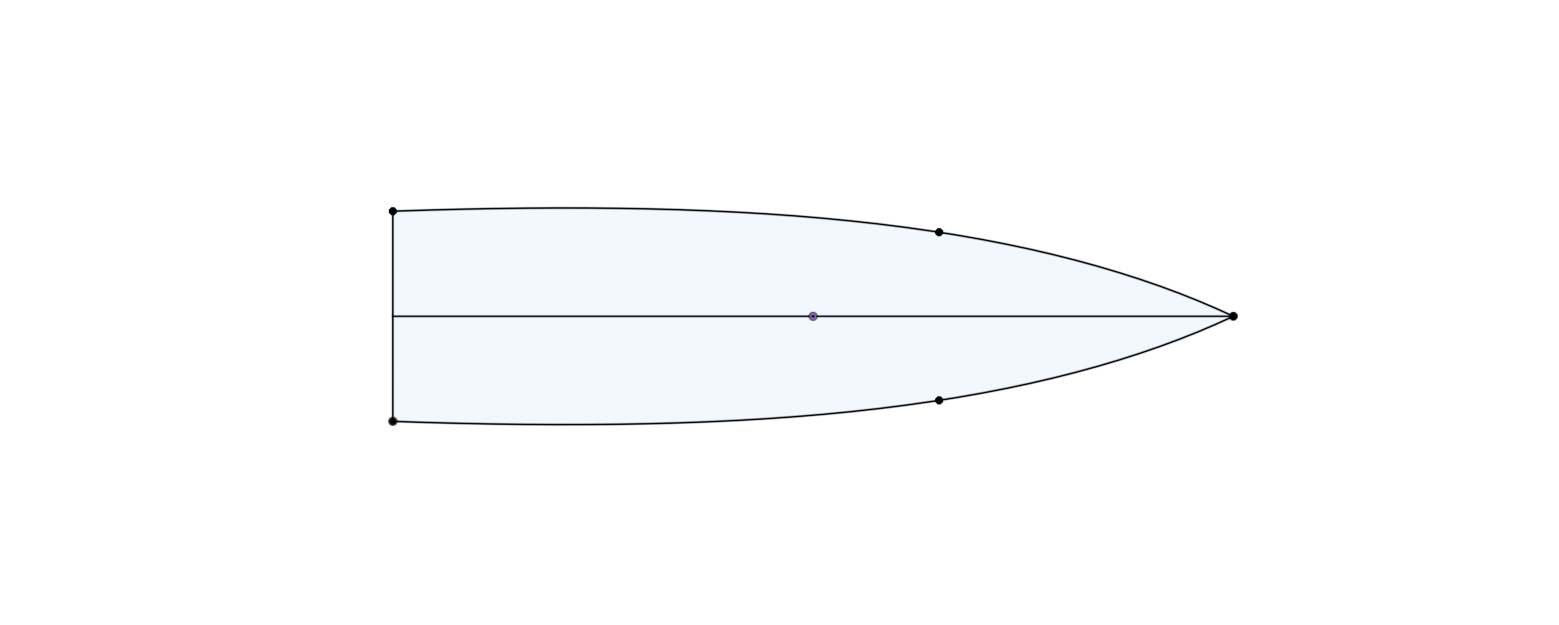
\includegraphics[width=\linewidth]{assets/boot sketch top.png}
        \caption{Topansicht des Boots}
        \label{fig:Decktop}
    \end{subfigure}
    \hfill
    \begin{subfigure}[b]{0.48\linewidth}
        \centering
        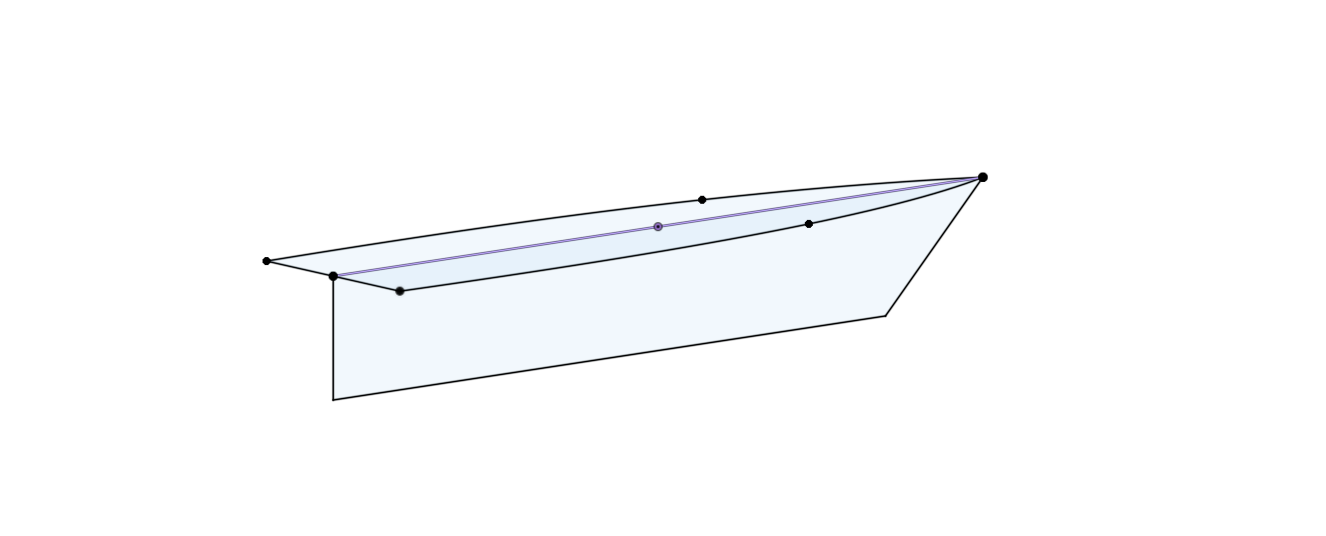
\includegraphics[width=\linewidth]{assets/boot_skizze_2.png}
        \caption{Seitenansicht mit Steven}
        \label{fig:Deckseite}
    \end{subfigure}

    \vskip\baselineskip

    % Untere Reihe
    \begin{subfigure}[b]{0.48\linewidth}
        \centering
        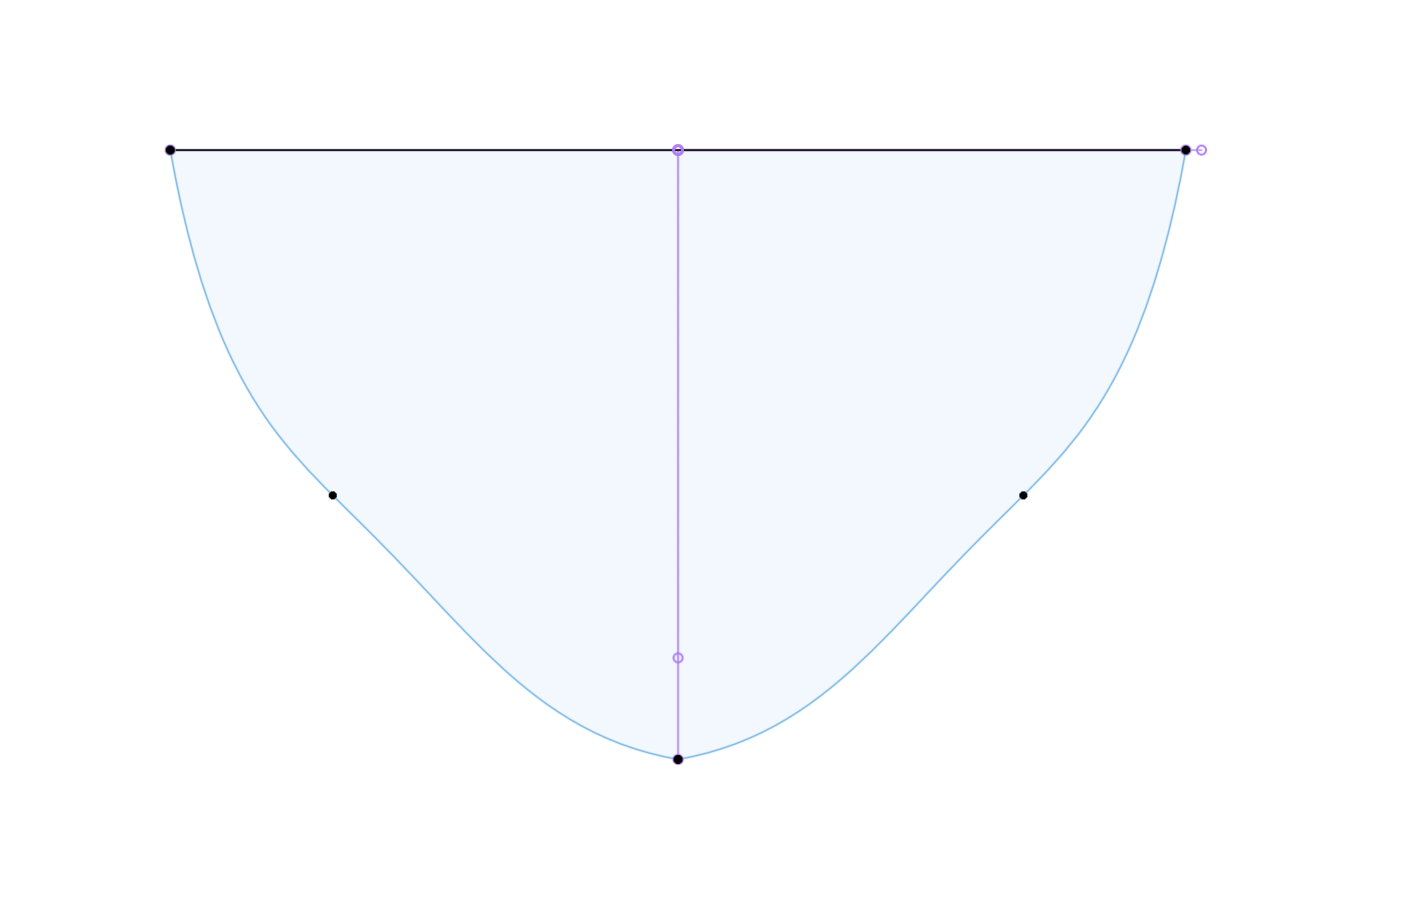
\includegraphics[width=\linewidth]{assets/Heck_boot.png}
        \caption{Heckansicht}
        \label{fig:Deckheck}
    \end{subfigure}

    \caption{Bootsansichten: Top-, Seiten- und Heckansicht}
    \label{fig:Bootsansichten}
\end{figure}


Mit dem Erhebungswerkzeug (Loft Tool) der CAD Software wird im Anschluss aus den zweidimensionalen Skizzen ein dreidimensionaler Körper berechnet.

Im Anschluss wird die Bootskörperform von de CAD Software mit einer Wandstärke von 4 cm innen ausgehöhlt.

\begin{figure}[H]
    \centering
    \begin{subfigure}[b]{0.48\linewidth}
        \centering
        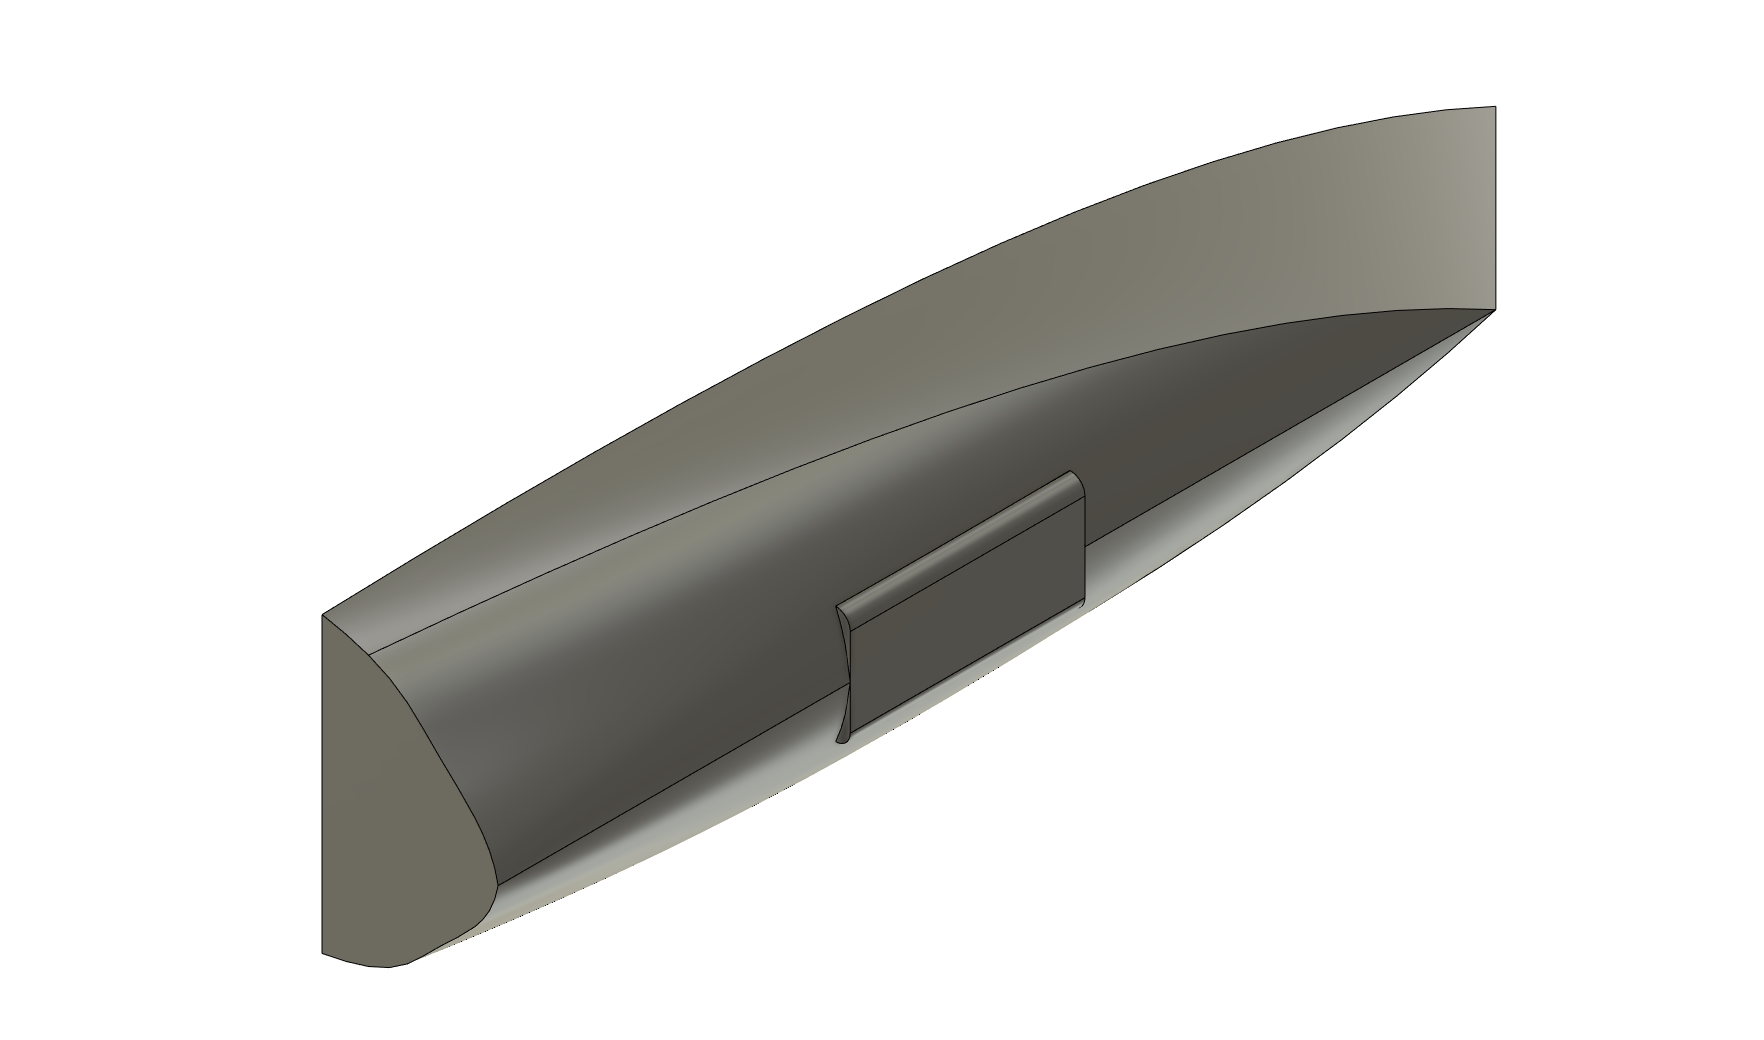
\includegraphics[width=\linewidth]{assets/kielbefestigung2image.png}
        \caption{Fläche zur Montage des Kiels}
        \label{fig:Kielmontage}
    \end{subfigure}
    \hfill
    \begin{subfigure}[b]{0.48\linewidth}
        \centering
        \includegraphics[width=\linewidth]{assets/Hohlkörper.png}
        \caption{Schnittbild Hohlkörper}
        \label{fig:Hohlkoerper}
    \end{subfigure}
    \caption{Darstellung der Kielmontagefläche und des Hohlkörper-Schnitts}
    \label{fig:Kiel_und_Hohlkoerper}
\end{figure}
Danach wird der bereits ausgehöhlte Körper auf zwölf Spanten mit einem einheitlichem Abstand je 14 cm reduziert. Die Spanten haben eine Stärke von 18 mm. Die Masse der Spanten verjüngen sich von der Mitte zum Bug und Heck hin.


Die hinterste Spannte, die Achtersteven genannt wird, ist nicht hohl, weil sie sich am Ende des Bootskörpers befindet und diesen abschliesst.

Mit Ausnahme der Spanten 5, 6 und 7 laufen die Spanten unten spitz zu. Die Spanten 5, 6 und 7 sehen einen flachen Boden von 15 cm vor, der dazu dient, später den Kiel des Bootes sicher und senkrecht zu befestigen.
\begin{figure}[H]
    \centering
    \begin{subfigure}[b]{0.6\linewidth}
        \centering
        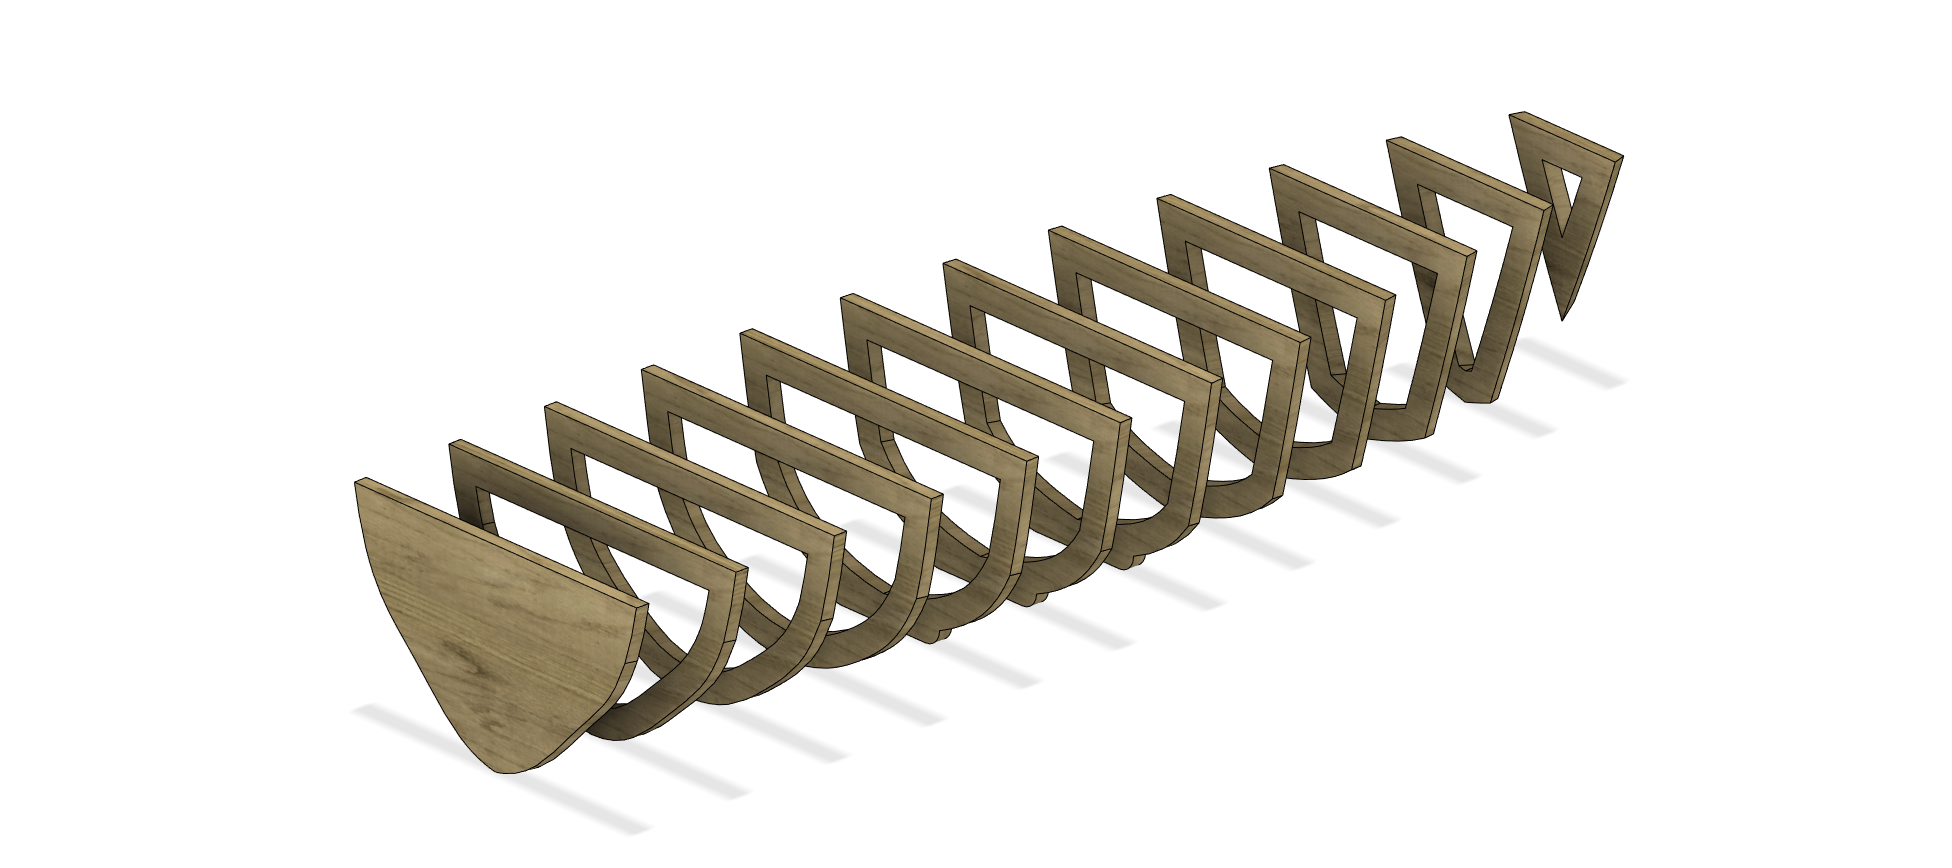
\includegraphics[width=\linewidth]{assets/rippen_cad.png}
        \caption{Spantenansicht}
        \label{fig:Spantenansicht}
    \end{subfigure}
    \hfill
    \begin{subfigure}[b]{0.38\linewidth}
        \centering
        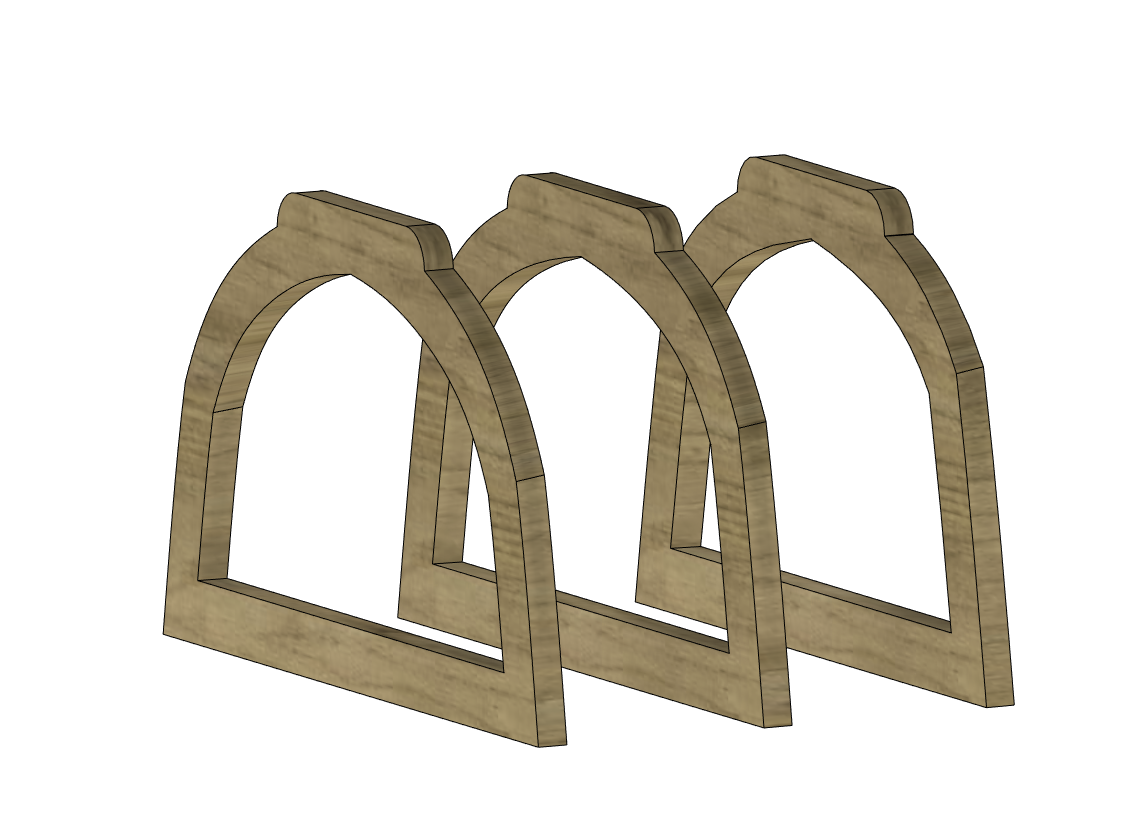
\includegraphics[width=\linewidth]{assets/spanent_upside_down.png}
        \caption{Spanten 5, 6 und 7}
        \label{fig:SpantenDetail}
    \end{subfigure}
    \caption{Spantenübersicht und Detailansicht der Spanten 5–7}
    \label{fig:SpantenUebersicht}
\end{figure}



Der Bug des Bootes läuft spitz zu. Diese Form der Spitze ist in Holz schwierig zu bauen. Es wird daher auf die klassische Konstruktion mit einer Bugspante verzichtet. An ihrer Stelle wird die gesamte Spitze im 3D Druckverfahren aus Kunststoff als ein einziges Werkstück gedruckt. Es wird mit der vordersten Spante verklebt. Der Bugspitz ist nicht in Massivbauweise, sondern als Hohlkörper vorgesehen.
\begin{figure}[H]
    \centering
    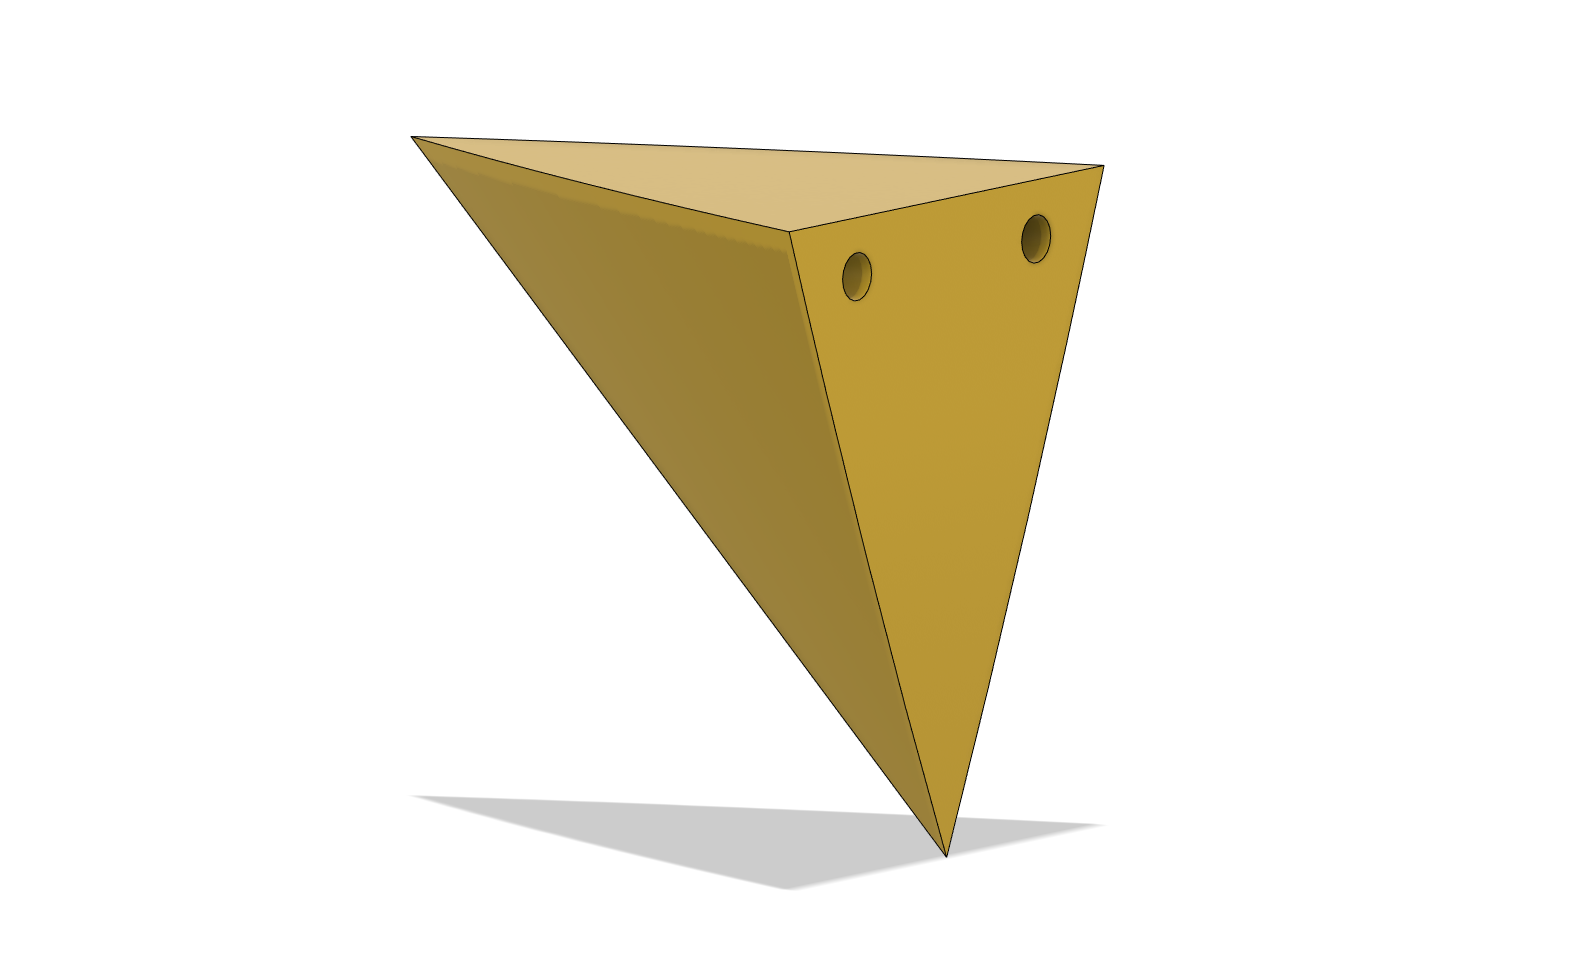
\includegraphics[width=0.5\linewidth]{assets/bug_spitz.png}
 \caption{Bugspitz}
    
\end{figure}
Die meisten Boote und Schiffe verfügen über einen mittschiffs im Boden angebrachten Längsverband, der das Rückgrat des Bootes bildet. An ihm sind die querstabilisierenden Spanten befestigt. Dieser Längsverband bildet zusammen mit einer vertikalen Unterwasserverlängerung den Kiel und mündet am Anfang und Ende in den Steven. 

Da für die vorliegende Konstruktion ein Flachdeck vorgesehen ist, der Boden des Schiffskörpers aber gewölbt ist, wird von dieser klassischen Kielkonstruktionsweise abgewichen. Die Längsverbindung der Spanten wird nicht am Boden des Schiffs, sondern direkt unter dem Deck vorgesehen. Sie besteht auch nicht aus einem einzelnen mittschiffs angebrachten Längsverband, sondern aus zwei Längsverbänden, die in einem Abstand von 10 cm von der Mittelachse parallel über die ganze Bootslänge horizontal angebracht werden. Sie bestehen aus zwei Alluminiumröhren mit einem Durchmesser von je 16 mm. Die beiden Röhren werden durch die Spanten geführt, in welchen im oberen Holm je zwei runde Löcher im Abstand von 10 cm gebohrt werden. Am vorderen Ende des Bootes werden die beiden Röhren in zwei dafür vorgesehene Hohlöffnungen des gedruckten Bugspitzes geführt und verklebt.

Diese Konstruktion ist viel einfacher zu bauen als ein klassischer Kielaufbau. Sie ist jedoch bei bemannten Booten nicht verbreitet, weil die beiden Längsverbindungen direkt unter dem Deck dem Einbau eines Cockpits im Weg stehen würden. Möglich wäre allein, das Cockpit auf dem Deck aufzubauen, was sowohl die Stabilität als auch den Komfort stark beeinträchtigen würde. Auch ein Zugang zu einer Kajüte würde verunmöglicht.
\begin{figure}[H]
    \centering
    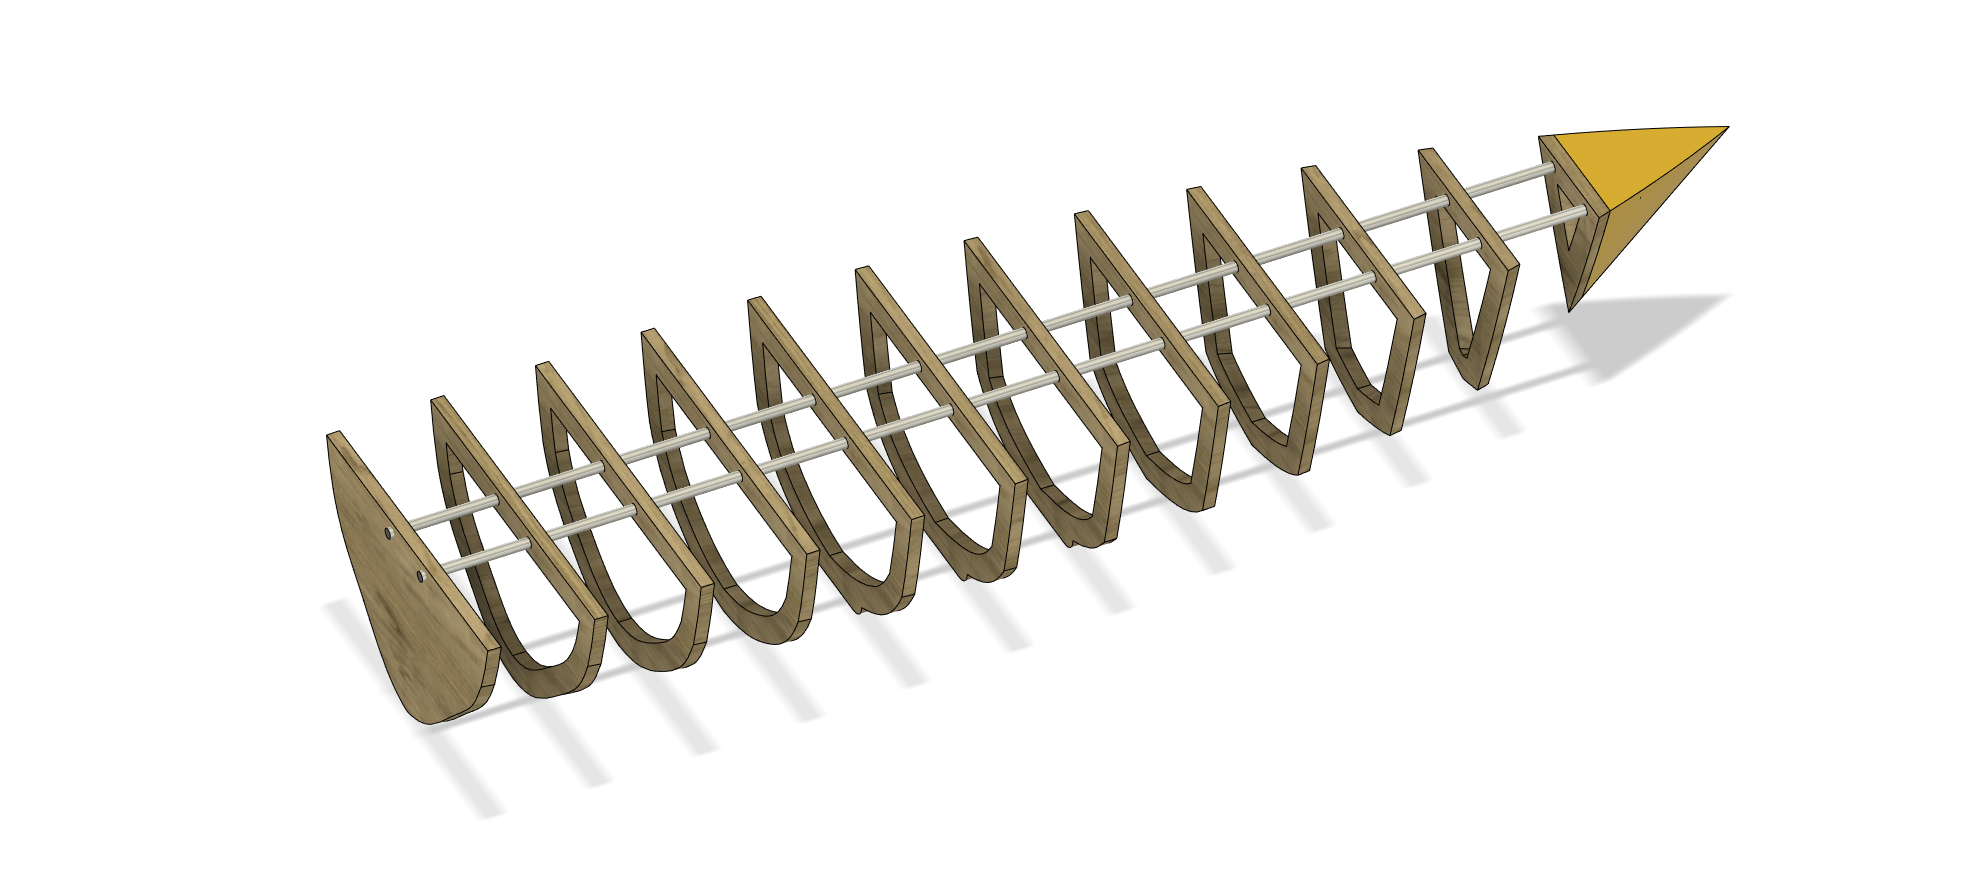
\includegraphics[width=1\linewidth]{assets/full_skellet.png}
    \caption{Abbild der Spanten und des Spitzes in Verbindung}
    
\end{figure}

%\begin{figure}[H]
%  \centering
%  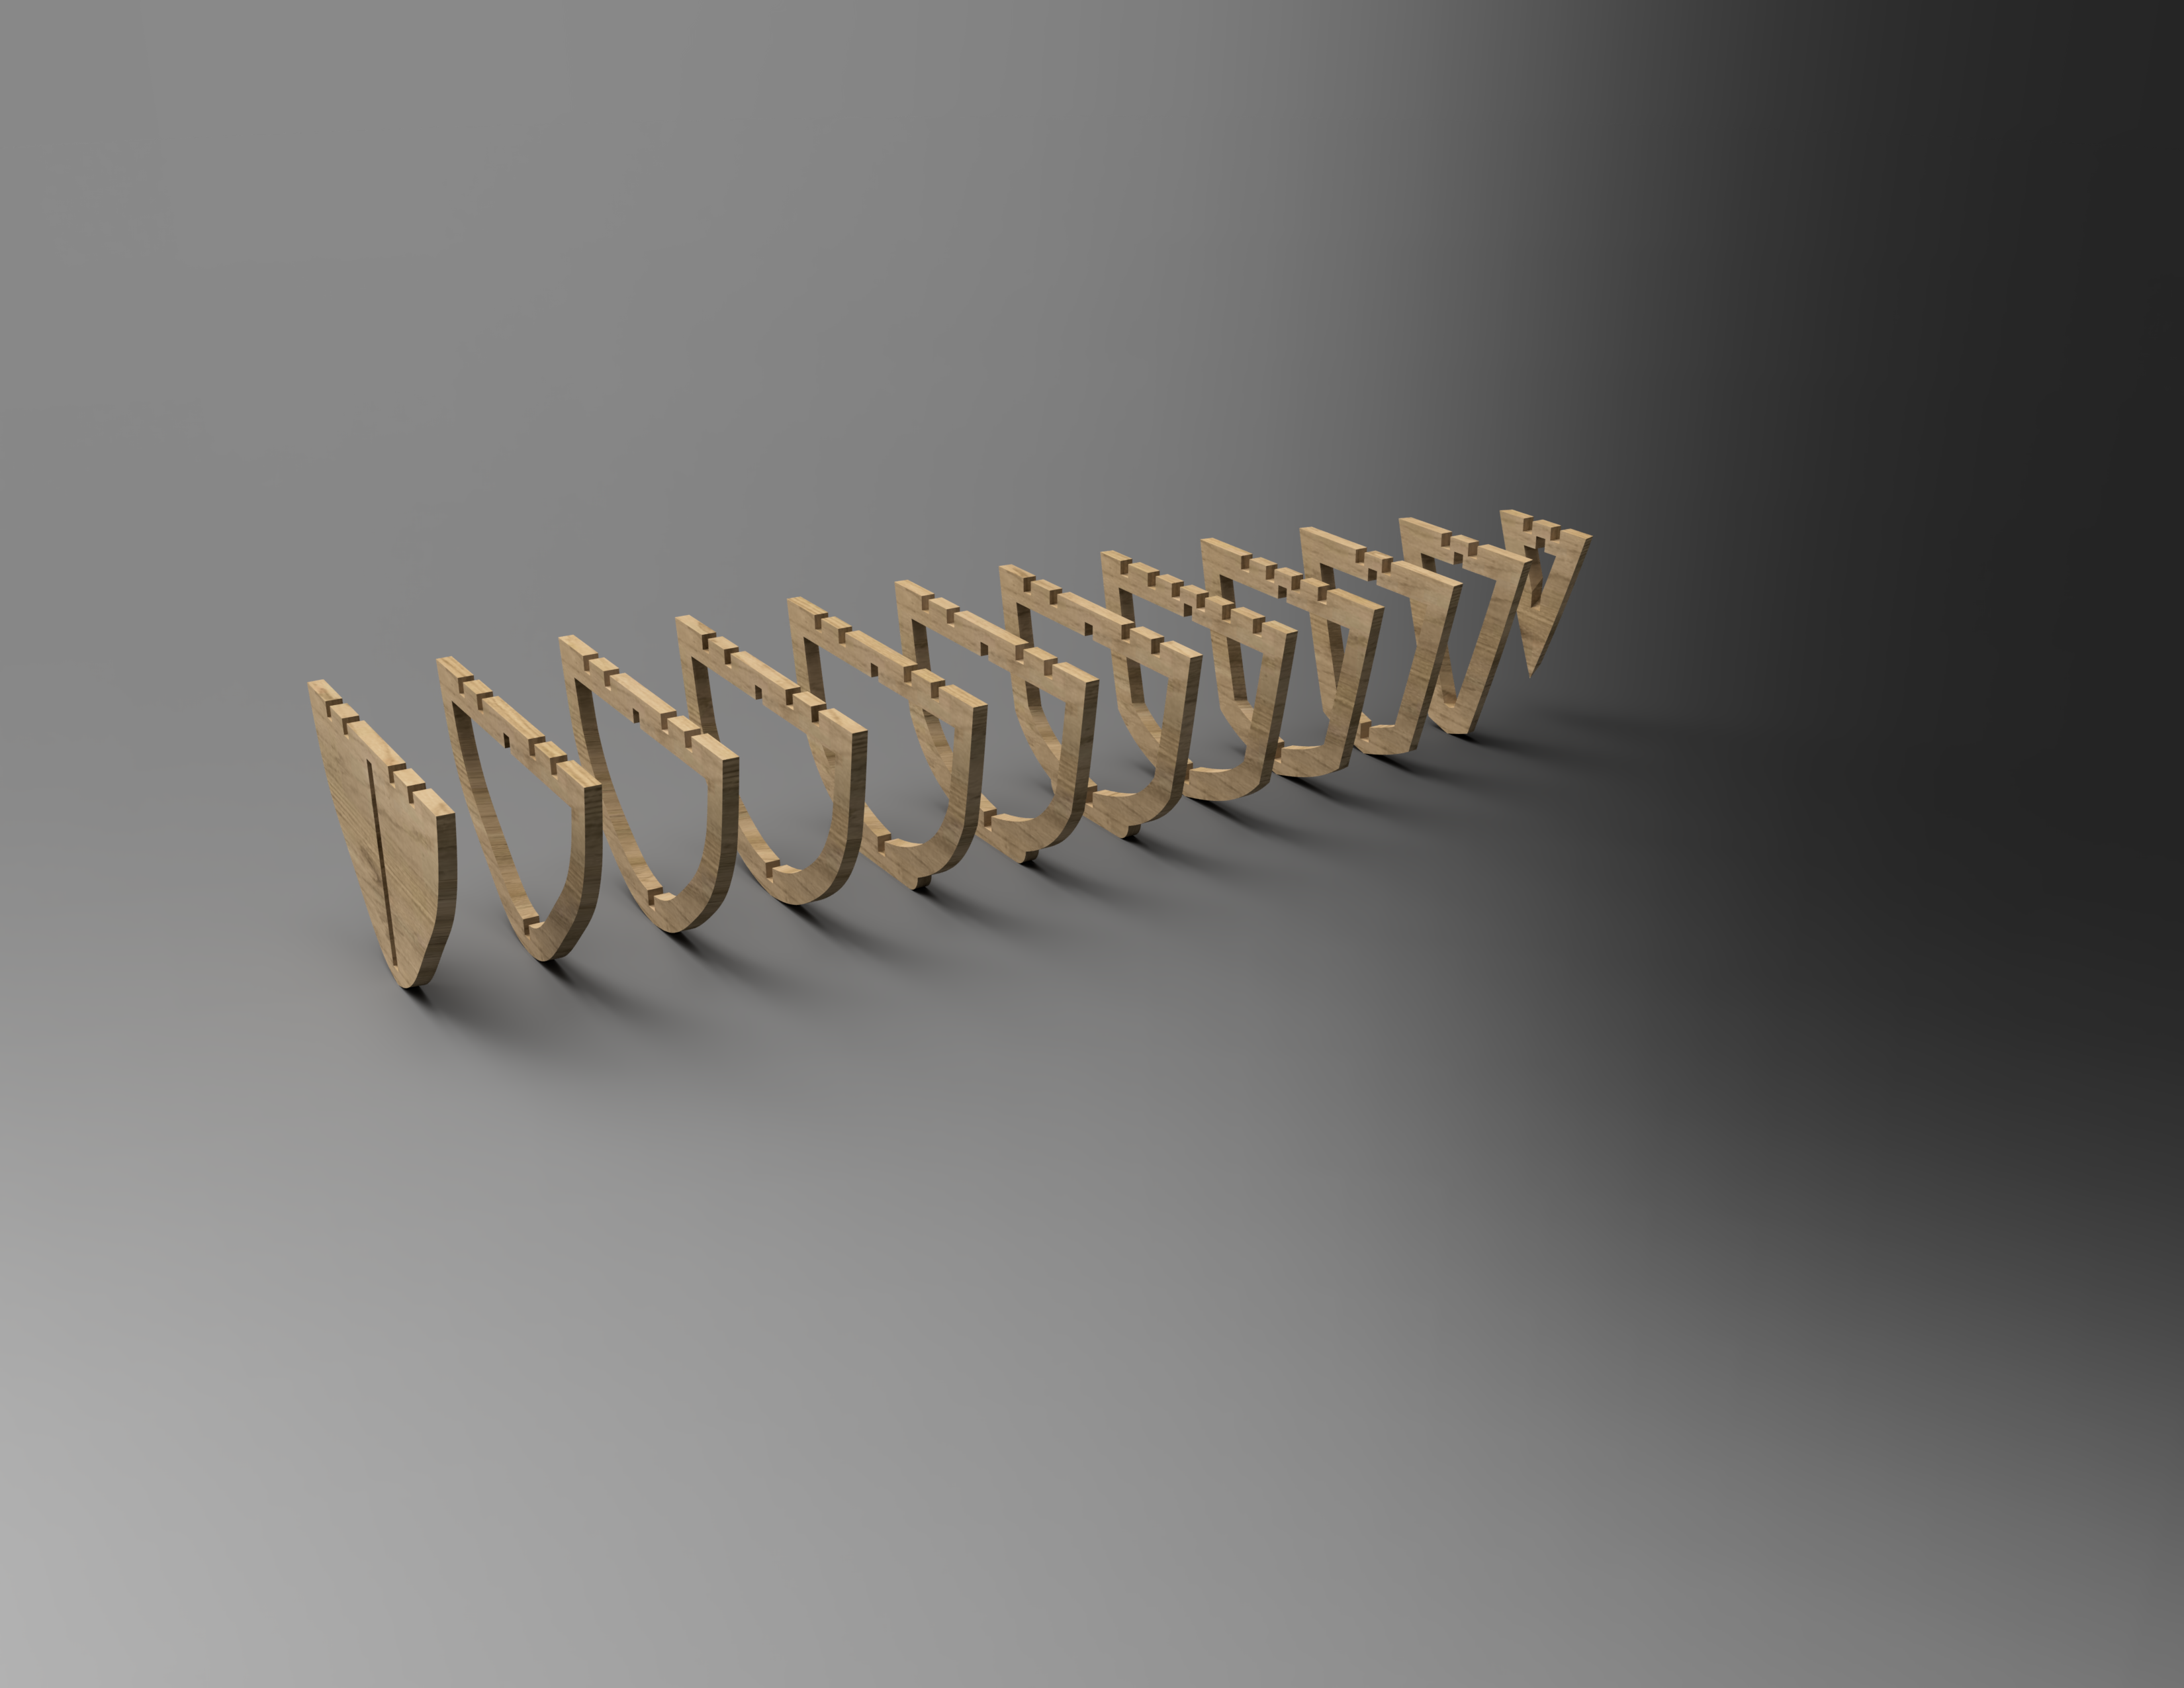
\includegraphics[width=\textwidth]{assets/rippenv1.png}
%  \caption{Render einer ersten Version des Rippenmusters (nicht Final) }
%  \label{fig:rippenv1}
%\end{figure}

\section{Konstruktion des Hauptsegels und des Sailflap}

\begin{figure}[H]
    \centering
    \begin{subfigure}[b]{0.43\linewidth}
        \centering
        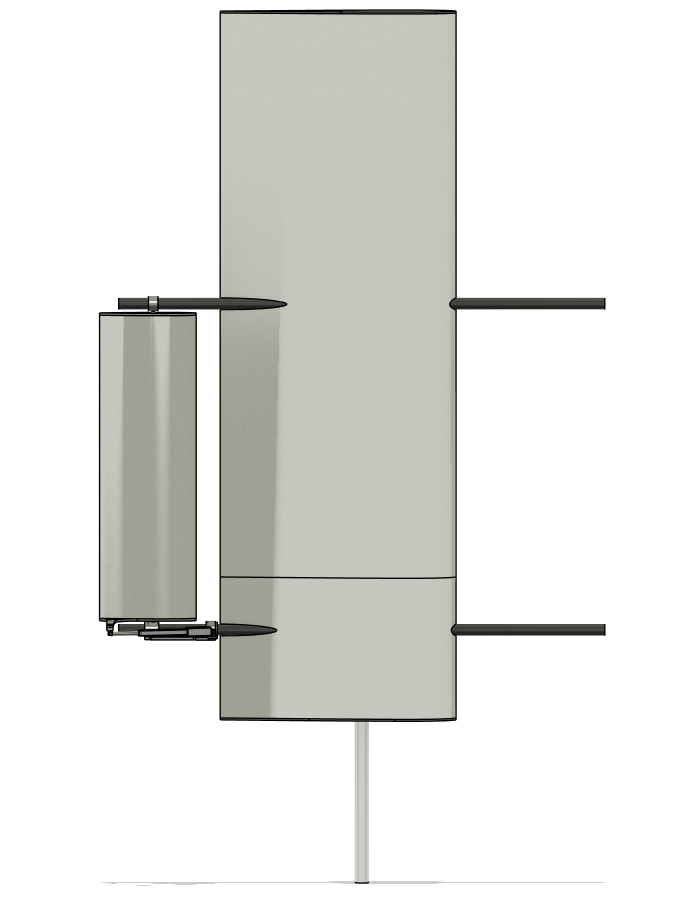
\includegraphics[width=\linewidth]{assets/sail_cad.png}
        \caption{CAD-Entwurf des Segels mit Sailflap}
        \label{fig:sailcad}
    \end{subfigure}
    \hfill
    \begin{subfigure}[b]{0.52\linewidth}
        \centering
        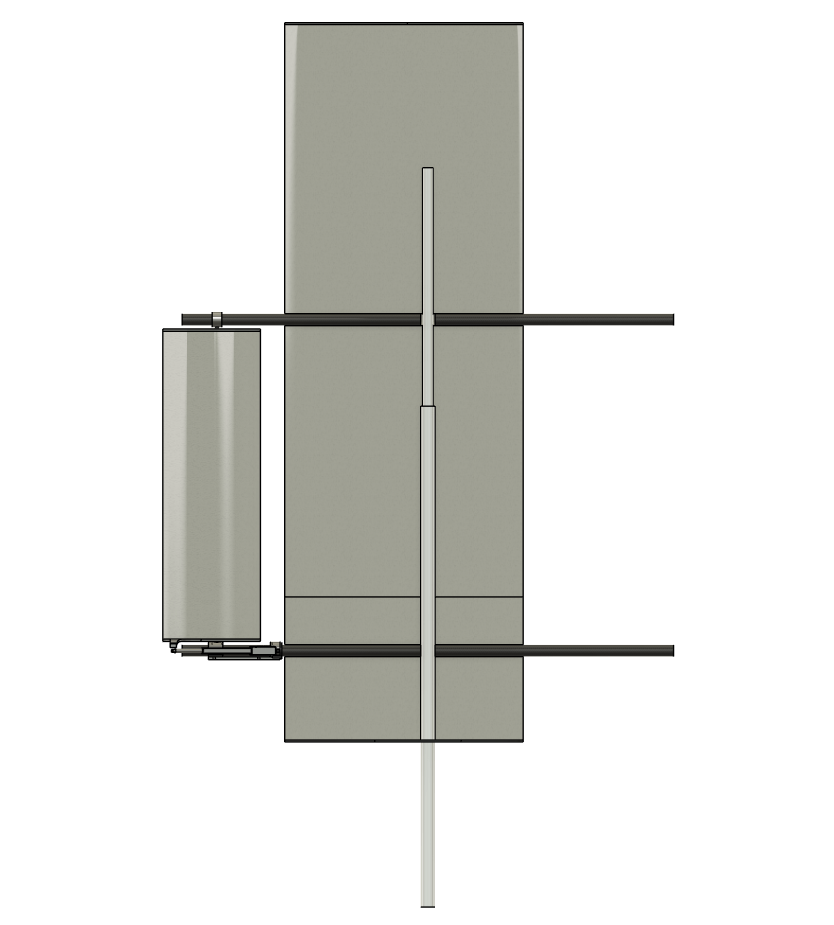
\includegraphics[width=\linewidth]{assets/sail_cad_inner.png}
        \caption{Innenansicht des Segels}
        \label{fig:sailinner}
    \end{subfigure}
    \caption{CAD-Darstellungen des Segels}
    \label{fig:segel_cad_multifig}
\end{figure}

Hauptsegel und Sailflap werden ebenfalls mit dem CAD Programm entworfen. 
\subsection{Hauptsegel}
Die grundlegende Form des Festsegels wurde aus der bereits erwähnten Arbeit  von Tretow übernommen \enquote{Design of a free-rotating wing sail for an autonomous sailboat} \cite{Tretow2017DesignOA}
Dabei wurde lediglich die aerodynamische Grundform, nicht aber der gesamte Segelaufbau übernommen.
Das Segel, welches in dieser Arbeit verwendet wird, verjüngt sich nur sehr bescheiden. Damit wird der spätere Herstellungsprozess stark vereinfacht. Nachteilig wirkt sich aus, dass wegen des deutlich grösseren oberen Teils des Segels wegen der Hebelkraft deutlich mehr Drehmoment auf das Boot einwirkt. Das könnte zu einer stärkeren Krängung führen. Da die Segelfläche jedoch insgesamt eher gering ist, ist davon auszugehen, dass sich dies nicht als grosses Problem erweisen wird.

Das Segel wird aus vier identischen Teilen zusammengesetzt, die aus Standard XPS Platten herausgeschnitten werden. Je zwei Teile müssen dann mit ihrer planen Seite verklebt werden, auf dass ein stromlinienförmiger Körper entsteht. Im vorderen Teil der beiden Segelteile wird in einer ausgeschnittenen Kerbe der Mast geführt. Dieser besteht aus einem Aluminiumrohr.
\subsection{Sailflap}
\label{sec:sailflap}
Das Sailflap hat dieselbe Form wie das Grosssegel, ist aber lediglich 645 mm lang. Das Sailflap wird mit zwei Carbonstangen am Grossssegel befestigt, welche einen Durchmesser von 25 mm haben. Mithilfe von 3D-gedruckten Teilen, welche in der Abbildung \ref{fig:sailmechanics} dargestellt werden, kann das Flap am Grosssegel befestigt werden.

Auf der Darstellung \ref{sail_mechanics_multiview} ist der Aktuator, der zur Änderung der Position des Sailflaps verantwortlich ist, zu sehen. Dieser ist an jeweils zwei 3D gedrucken Teilen verbunden. Zum einen an der Carbonstange mit zwei Befestigungspunkten. Zudem ist er mit dem Sailflap verbunden. Der Abstand zwischen Befestigungspunkt und Aktuator lässt sich damit erklären, dass sich das Flap in beide Richtungen drehen muss.

\begin{figure}[H]
    \centering
    \begin{subfigure}[b]{0.48\linewidth}
        \centering
        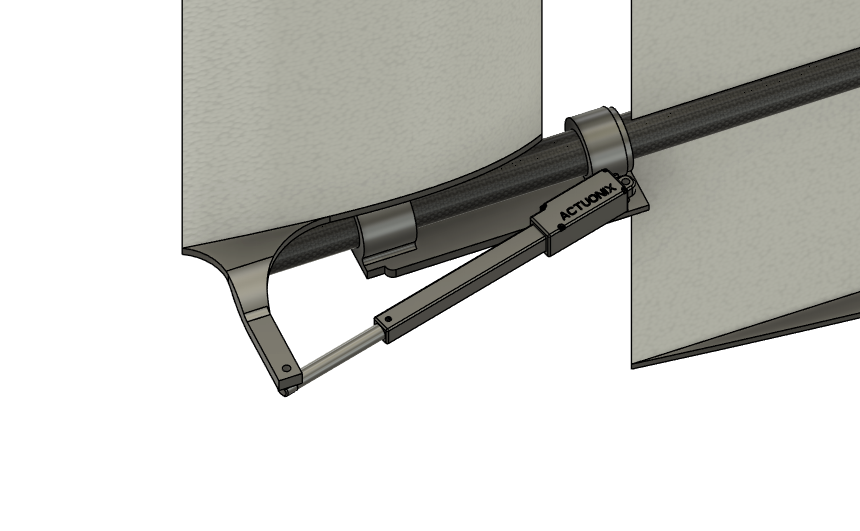
\includegraphics[width=\linewidth]{assets/sail_mechanics.png}
        \caption{Befestigung und Mechanik des Sailflaps (Seitenansicht)}
        \label{fig:sailmechanics}
    \end{subfigure}
    \hfill
    \begin{subfigure}[b]{0.48\linewidth}
        \centering
        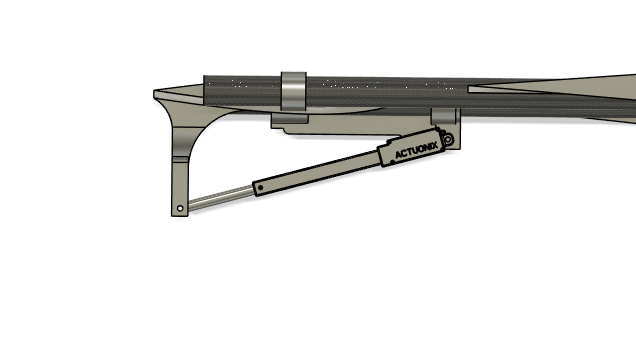
\includegraphics[width=\linewidth]{assets/salimech_top.png}
        \caption{Befestigung und Mechanik des Sailflaps (Draufsicht)}
        \label{fig:sailmechanics_top}
    \end{subfigure}
    \caption{Mechanische Konstruktion des Sailflaps in Seiten- und Draufsicht}
    \label{fig:sail_mechanics_multiview}
\end{figure}


\begin{figure}[H]
    \centering
    \begin{subfigure}[b]{0.28\linewidth}
        \centering
        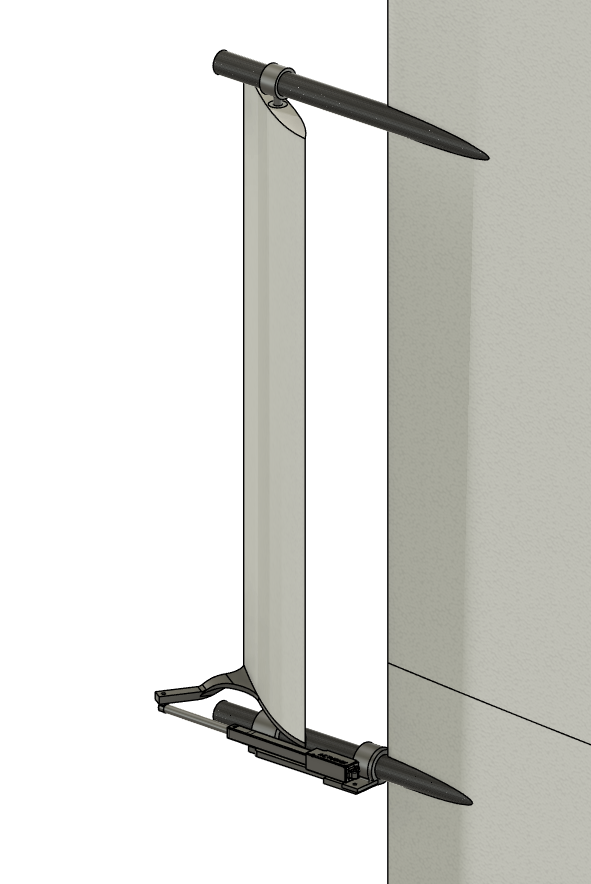
\includegraphics[width=\linewidth]{assets/flap_tilt_1.png}
        \caption{Flap in Position A}
        \label{fig:flaptilt1}
    \end{subfigure}
    \hfill
    \begin{subfigure}[b]{0.28\linewidth}
        \centering
        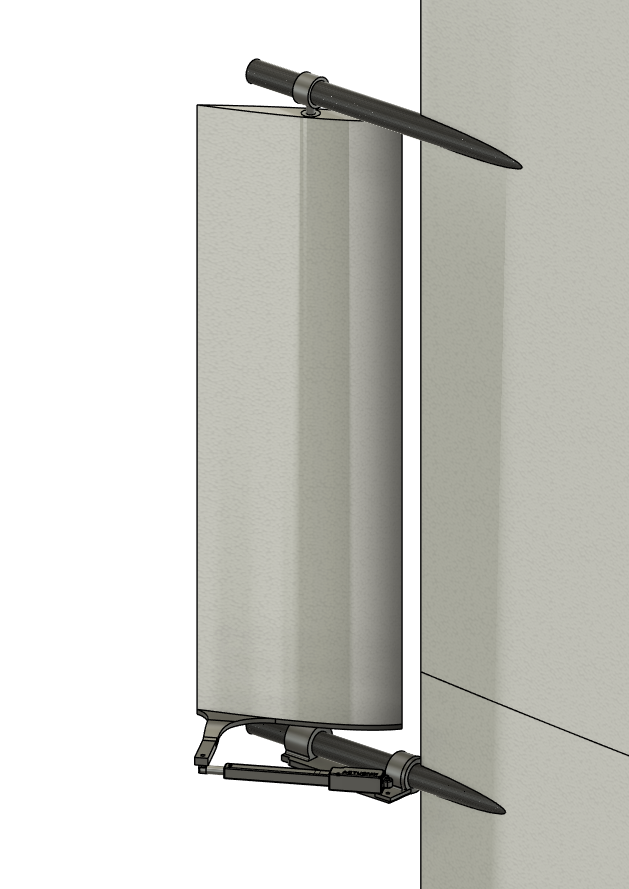
\includegraphics[width=\linewidth]{assets/flap_tilt_2.png}
        \caption{Flap in Position B}
        \label{fig:flaptilt2}
    \end{subfigure}
    \caption{Vergleich der Flap-Neigungspositionen}
    \label{fig:flaptilt_comparison}
\end{figure}


\section{Konstruktion des Kiels}

\begin{figure}[H]
    \centering
    \begin{subfigure}[b]{0.51\linewidth}
        \centering
        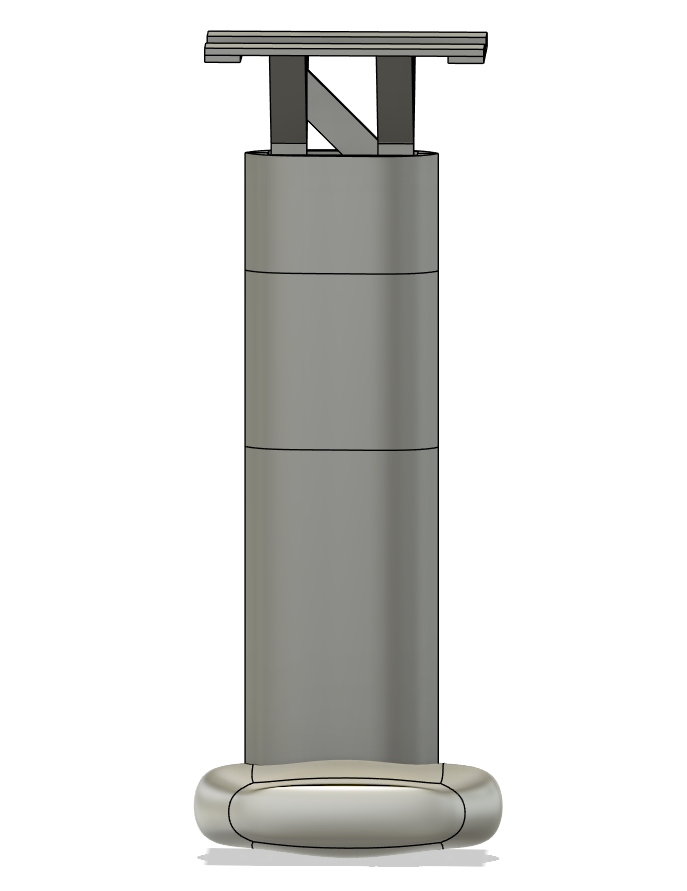
\includegraphics[width=\linewidth]{assets/kiel_1.png}
        \caption{Kiel mit Hydroshell}
        \label{fig:kiel1}
    \end{subfigure}
    \hfill
    \begin{subfigure}[b]{0.39\linewidth}
        \centering
        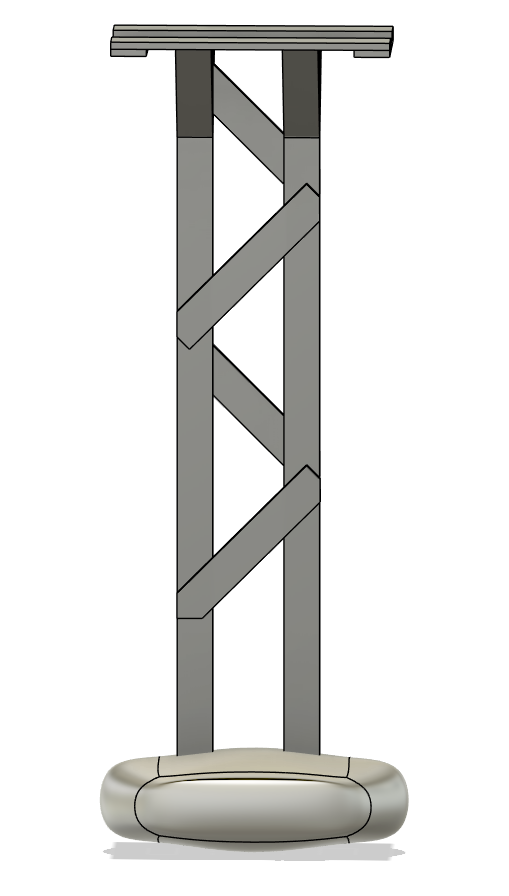
\includegraphics[width=\linewidth]{assets/kiel_2.png}
        \caption{Kiel ohne Hydroshell}
        \label{fig:kiel2}
    \end{subfigure}
    \caption{Unterschiedliche Zustände der Kielanordnung}
    \label{fig:kiel_comparison}
\end{figure}



Oben wird bei der Beschreibung der Konstruktion des Bootskörpers ausgeführt, dass von der klassischen Bauweise mit einem über die gesamte Länge des Bootes reichenden Kiel abgewichen wird. Es gibt keine über die gesamte Länge des Schiffsbodens reichende Längsverbindungen. Dafür haben die Formen der Spanten 5, 6 und 7, wie ebenfalls bereits oben ausgeführt, einen flachen Boden. Das ist so vorgesehen, damit der Kiel stabil an den Spanten befestigt werden kann.

Der Kiel besteht grundsätzlich aus einer inneren, verschweissten Fachwerkstruktur. Diese soll dem 610 mm langem Kiel die nötige Stabilität geben. Wie auf der Grafik ersichtlich, sind die Verbindungsstücke jeweils alternierend auf beiden Seiten verbaut.

Als Balast dient eine Wasserwiederstands minimierende Blechform, welche mit Blei gefüllt wird. Diese ist mit der Stahlstruktur verschweisst. 

Im oberen Teil, der mit dem Boot verbunden verschraubt wird ist eine zusätzliche Verstärkung verbaut. Dies kommt daher, dass die Kraftübertragung und die Momente aufgrund des langen Hebels des Kiels dort Maximal sind. Ein Versagen des Kiels wäre Katastrophal. 

Verschraubt wird der Kiel mit 4x M12 Schrauben an eine sich im Boot befindende Stahlprofile. 

Überdeckt wird der Kiel mit 3D gedruckten Kunststoffprofilen welche mit Bezière Kurven angefertigt wurden. Diese sind jedoch nur Form tragend, denn diese werden mit zwei schichten Glasfasermatten überdeckt.

Hohlräume werden mit Wasserfestem Bauschaum gefüllt um das eindringen von Wasser und die damit kommende Korrosion zu vermeiden. Der Kiel ist komplett luftdicht verschlossen. Das in Abbildung  \ref{fig:kiel1} Loch im oberen des Kiels wird mit Schaum gefüllt und Glasfasermatten überdeckt. Es ist kein Kunststoffteil notwendig. 


\begin{figure}[H]
    \centering
    \begin{subfigure}[b]{0.48\linewidth}
        \centering
        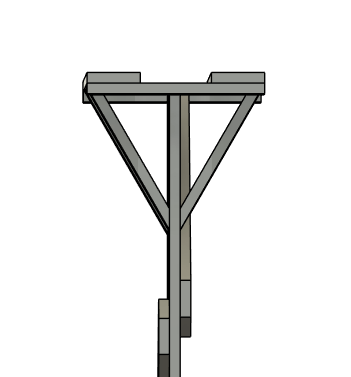
\includegraphics[width=\linewidth]{assets/kiel_side1.png}
        \caption{Kiel Ansicht 1}
        \label{fig:kiel_side1}
    \end{subfigure}
    \hfill
    \begin{subfigure}[b]{0.48\linewidth}
        \centering
        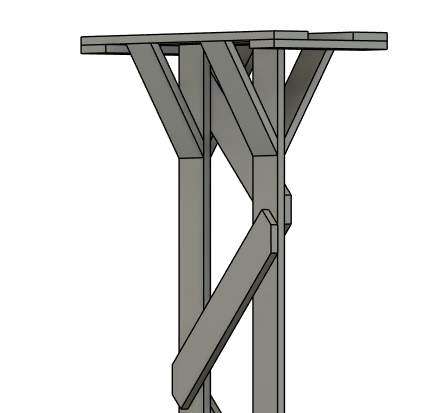
\includegraphics[width=\linewidth]{assets/kiel_side2.png}
        \caption{Kiel Ansicht 2}
        \label{fig:kiel_side2}
    \end{subfigure}
    \caption{Seitenansicht des Kiels in zwei verschiedenen Zuständen}
    \label{fig:kiel_side_views}
\end{figure}



\section{Konstruktion des Ruders}
Das Runder, welches zur Steuerung des Bootes verstnwortlich ist, wird wie die übrigen tragenden Holzteile des Boots ebenfalls aus Tannen-Leimholzplatten gesägt.

Die dem Boot zugewandte Seite des Ruders wird in eine elliptische Form geschliffen, da damit verbesserte hydrodynamische Eigenschaften erhofft werden. Dazu wurden aber keine weiteren Analysen oder Simulationen durchgeführt, da in diese Arbeit kein Fokus auf ein optimales Strömungsverhalten gelegt wird.

Zur Befestigung des Ruders am Bootskörper wird ein Befestigungsstück mittels 3D Druck Verfahren hergestellt. Dieses wird mit PETG gedruckt, da das Material deutlich stärker ist als das sonnst verwendete PLA. Durch die sichtbaren Löcher werden Schrauben durchgeführt und verschraubt. 

\begin{figure}[H]
    \centering
    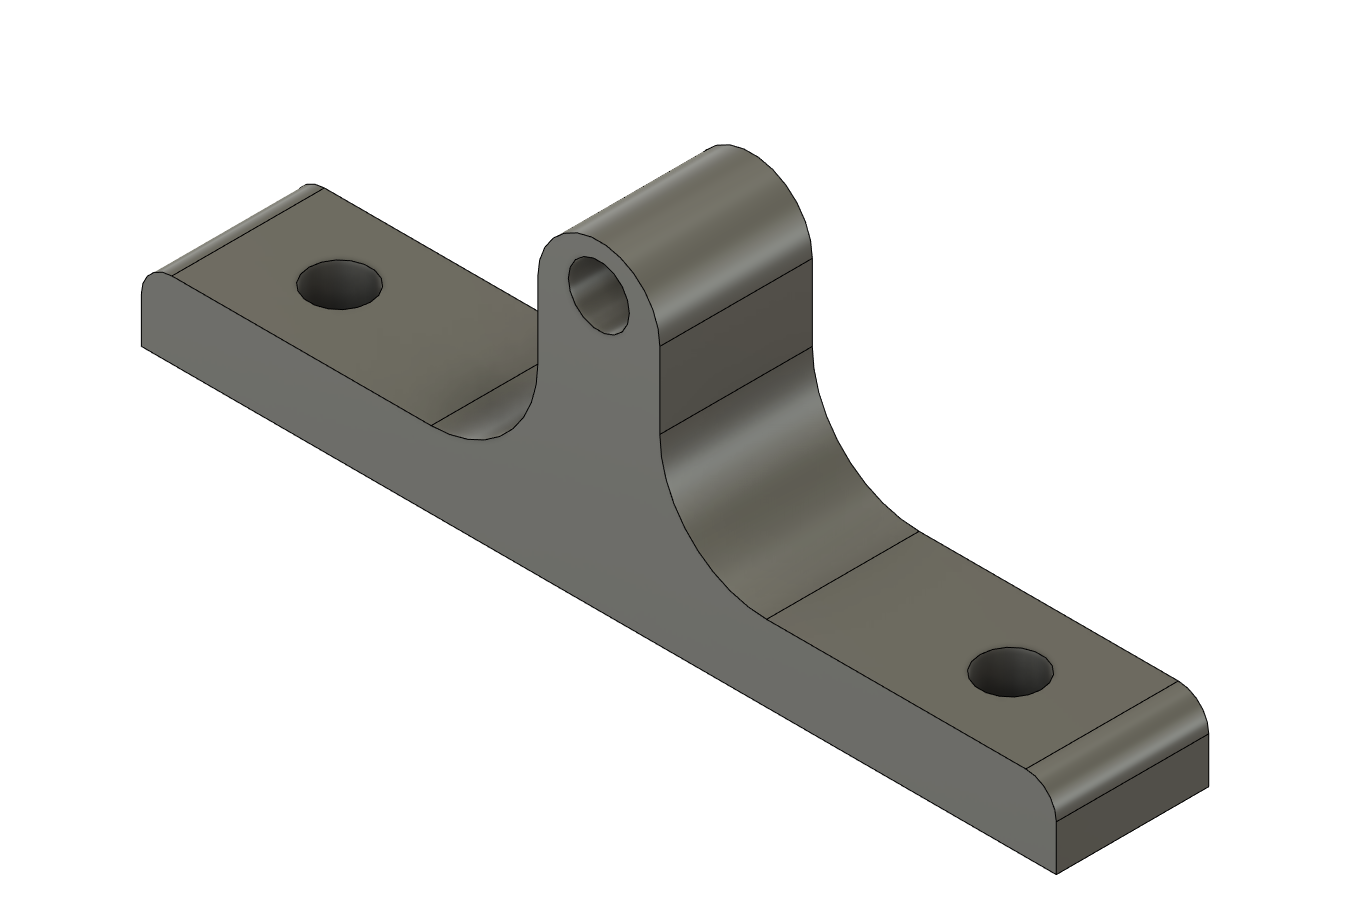
\includegraphics[width=0.3\linewidth]{assets/rudder_connector_image.png}
    \caption{Aktuator Befestigung}
    
\end{figure}